%-----------------------------------------------------------------------------------------------------------------
\chapter[Construção da \textit{pipeline} de integração contínua]{Construção da \textit{pipeline} de integração contínua}
\label{Ch:CapExemplo}
%-----------------------------------------------------------------------------------------------------------------
\section{Estudo de viabilidade das \textit{frameworks} de teste}
\label{Ch:OutroCap}

\hspace{1cm}Uma das vantagens da implementação de uma \textit{pipeline} de testes automatizada é a redução do tempo de validação e entrega de código funcional. Para que o código esteja funcional é necessário que, em primeiro lugar, corresponda aos requisitos para o qual está a ser desenvolvido. Uma vez verificada a funcionalidade -- e tendo sido verificado que os seus requisitos estão de acordo com as expectativas iniciais -- podemos então pensar no segundo ponto que consiste na otimização da \textit{pipeline}, isto é, na redução da duração do tempo de compilação dos projetos, dos testes e de outros processos. Sabendo que existem várias \textit{frameworks} à disposição, dependendo da linguagem de programação utilizada para desenvolvimento, foram escolhidas aquelas que se melhor se ajustam ao contexto da execução dos testes.


\hspace{1cm}No desenvolvimento orientado a testes há uma metodologia de organização e estruturação do código bastante interessante, que é dividida em três fases: \textit{Arrange, Act} e \textit{Assert}. Esta abordagem aos testes é conhecida no mundo da programação como AAA ou \textit{triple A}.

\subsection{\textit{Arrange, Act \& Assert}}

\hspace{1cm}Na primeira fase, \textbf{\textit{Arrange}}, apenas temos o código necessário para o \textit{setup} daquele \textit{test case}. É aqui que são criados os objetos ou \textit{mocks} (caso existam) e também é nesta fase que é definido o resultado esperado. Na segunda fase, \textbf{\textit{Act}}, é onde normalmente são invocados os métodos que vão ser testados. Na última fase, \textbf{\textit{Assert}}, vai ser verificado se o resultado obtido na execução das duas fases anteriores vai de encontro ao resultado esperado. Na figura \ref{Fig:Fig7} encontra-se um exemplo de uma classe de teste desenvolvida em \textbf{MSTest}. Esta classe de teste tem três \textit{test cases} diferentes e todos verificam que o resultado obtido é igual ao resultado esperado.

\begin{figure}[hbt!]
\centering
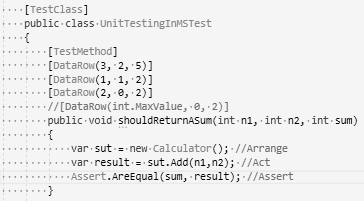
\includegraphics[width=0.5\linewidth]{Cap5/TestClass.png}
\caption{Exemplo de uma classe de teste}
\label{Fig:Fig7}
\end{figure}

\hspace{1cm}De seguida, para dar início a esta \textit{guideline}, irá ser delineada a estratégia para a execução dos testes num contexto próximo da realidade. Para tal, foi verificada, através do desenvolvimento de testes unitários, a funcionalidade da soma de dois números inteiros e foi verificado também que caso exista um número \textit{null} a soma não será executada. Este procedimento foi executado em cada \textit{framework} de testes e terá vários cenários de teste, dentro do mesmo contexto, com objetivos semelhantes.
\hspace{1cm}Tendo em conta que o desenvolvimento será orientado aos testes, será dado início através da criação de um projeto de teste. O tipo de \textit{framework} selecionada para o primeiro desenvolvimento é indiferente pelo que fica à escolha do leitor. No entanto, para estudar a viabilidade de cada uma das \textit{frameworks} de teste, foi utilizado:
\begin{itemize} 
  \item \textbf{C\#}, mais concretamente, \textbf{dotnet core} v2.2;
  \item Test Frameworks: \textbf{xUnit (2.4.0)}, \textbf{NUnit (3.11.0)} e \textbf{MSTest (1.4.0)};
\end{itemize}

\hspace{1cm}A classe que se pretende implementar apenas possui um método de adição que aceita dois inteiros caso sejam \textit{non-nullable} e retorna o valor da soma de ambos. É um método simples, cujo objetivo é somente a validação da funcionalidade de teste para permitir posterior utilização numa aplicação mais complexa.

\hspace{1cm}A solução contém o projeto \textbf{\textit{ModelClasses}} que mais tarde será o \textit{package} -- com a classe \textit{Calculator} -- juntamente com os três projetos de teste das três diferentes \textit{frameworks} (\ref{Fig:Fig8}).

\begin{figure}[hbt!]
\centering
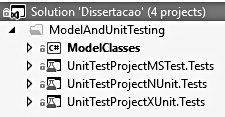
\includegraphics[width=0.35\linewidth]{Cap5/SolutionStructure.png}
\caption{Estrutura da solução}
\label{Fig:Fig8}
\end{figure}

\subsection{Tempo de execução dos testes}

\hspace{1cm}O tempo de execução das \textit{frameworks} de teste ($t_{n}$) será medido através de 9 tentativas. Este intervalo de tempo será estimado em milissegundos e será feita a média de tempo de execução para cada uma das \textit{frameworks}.

\begin{center}
 \begin{tabular}{||c | c | c | c | c | c | c | c | c | c | c ||} 
 \hline
 \textit{Framework} & \textit{$t_{1}$} & \textit{$t_{2}$} & \textit{$t_{3}$} & \textit{$t_{4}$} & \textit{$t_{5}$} & \textit{$t_{6}$} & \textit{$t_{7}$} & \textit{$t_{8}$} & \textit{$t_{9}$} & Média (ms)\\ [0.5ex] 
 \hline\hline
 MSTest & 87 & 79 & 90 & 86 & 90 & 88 & 86 & 100 & 116 & 91,33\\ 
 \hline
 NUnit & 76 & 59 & 58 & 60 & 55 & 55 & 64 & 60 & 56 & 60,33\\
 \hline
 XUnit & 62 & 50 & 42 & 54 & 44 & 43 & 53 & 46 & 48 & 49,11\\ [1ex] 
 \hline
\end{tabular}
\end{center}

\hspace{1cm}A \textit{framework} de teste com melhor performance foi o \textbf{XUnit} com um tempo médio de execução de testes de 49,11 (ms), seguido pelo \textbf{NUnit} com um tempo médio de execução de 60,33 (ms) tendo ficado o \textbf{MSTest} em último lugar, com um tempo médio de execução de 91,33 (ms). O tempo de testes foi retirado do tempo calculado pelo \textbf{IDE}, neste caso o \textit{Visual Studio 2017}, como pode ser visto na figura \ref{Fig:Fig9}.

\begin{figure}[hbt!]
\centering
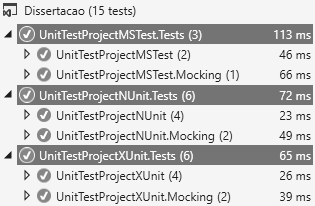
\includegraphics[width=0.5\linewidth]{Cap5/TestExplorer.png}
\caption{Explorador de testes do \textit{Visual Studio 2017}}
\label{Fig:Fig9}
\end{figure}

\subsection{Considerações}

\hspace{1cm}A empresa utiliza atualmente \textbf{MSTest} como \textit{framework} para desenvolvimento de testes. No entanto, a utilização de \textbf{XUnit} representaria uma melhoria de aproximadamente 46\% no tempo médio de execução de testes. Já a utilização de \textbf{NUnit} representaria uma melhoria de aproximadamente 34\% no tempo médio de execução de testes. Tendo em conta que o \textbf{MSTest} foi a \textit{framework} com pior performance e estando à disposição no mercado mais do que uma solução \textit{open-source} com performance evidentemente superior, o tempo de execução dos testes unitários pode ser otimizado quer com a utilização de \textbf{XUnit}, quer com a utilização de \textbf{NUnit}.

\hspace{1cm}Sendo o próximo objetivo a construção de uma \textit{pipeline} de integração e entrega contínua, que implica o desenvolvimento de testes de integração e performance, foi necessário eleger uma \textit{framework} para o seu desenvolvimento. Uma vez que se está ainda dentro da temática dos testes, ficou decidido -- juntamente com a orientação -- que seria utilizado \textbf{XUnit} daqui em diante, no desenvolvimento dos testes de integração, dada a sua rapidez de execução.

\section{Construção da \textit{pipeline} de integração contínua}

\hspace{1cm}Neste capitulo foi anteriormente desenvolvido um módulo de soma de dois números inteiros, através da utilização de \textbf{TDD}. Neste segmento, vai ser explicado todo o processo de criação de testes unitários e implementação de funcionalidades através da utilização de \textbf{XUnit} como \textit{framework} de desenvolvimento orientado a testes. De seguida, será delineado o processo de criação da \textit{pipeline}, com a comunicação com o sistema de controlo de versões (\textbf{GitLab}) em primeiro lugar, seguida pelo desenvolvimento da funcionalidade e da comunicação com \textbf{Jenkins} via \textbf{SSH}. Por último serão iniciadas duas instâncias, uma do \textbf{Nexus Repository OSS} e outra do \textbf{SonarQube} que serão o repositório de artefactos e ferramenta de análise estática respetivamente.

\subsection{Configuração do sistema de controlo de versões}

\hspace{1cm}A configuração dos repositórios varia consoante o tipo de projeto. Para este caso, em particular, é pretendido implementar-se uma \textit{pipeline} de testes automatizada com execução de testes unitários, análise estática, \textit{packaging} e \textit{push} da funcionalidade para um repositório remoto. Como vai ser necessário um repositório \textbf{.git}, onde será publicado o código da funcionalidade desenvolvida em formato não executável, faz sentido dar-se início pela comunicação entre o ambiente integrado de desenvolvimento -- onde é desenvolvida a funcionalidade -- e o repositório online que vai armazenar o código. 
\subsubsection{Criação de \textit{SSH keys}}

\hspace{1cm}Como foi explicado anteriormente, a comunicação via \textbf{SSH} exige que seja criado um \textit{key pair}. Para se criar o par de chaves, depois de estar instalado o \textbf{.git}, abre-se a linha de comandos, o \textbf{Git Bash}, e executa-se a instrução de criação de chaves  \colorbox{gray}{\textcolor{white}{\$ ssh-keygen -t rsa -b 4096 -C e-mail@exemplo.com}} que vai criar uma chave nova, utilizando o e-mail providenciado como um parâmetro de configuração que é único para cada utilizador. De seguida somos solicitados a dar um nome ao ficheiro onde se pretende guardar a chave recentemente criada e, caso se pressione \textit{Enter}, será utilizada a localização por defeito para guardar ficheiros. Com o destino seja validado, somos novamente solicitados, desta vez para criar uma password e reinserir a password. Quando o processo de criação do par de chaves é bem sucedido, é gerada uma \textit{fingerprint}, com uma imagem \textit{randomart} como mostrado na figura \ref{Fig:Fig10}. 

\hspace{1cm}Deste processo resultam dois ficheiros, um ficheiro contém a chave privada e outro contém a chave pública. A chave pública irá ser utilizada pelo \textbf{GitLab} para comunicar com a máquina onde está instalada a instância do \textbf{Jenkins} . A chave privada deve ser armazenada de forma segura \cite{gitssh}.

\begin{figure}[hbt!]
\centering
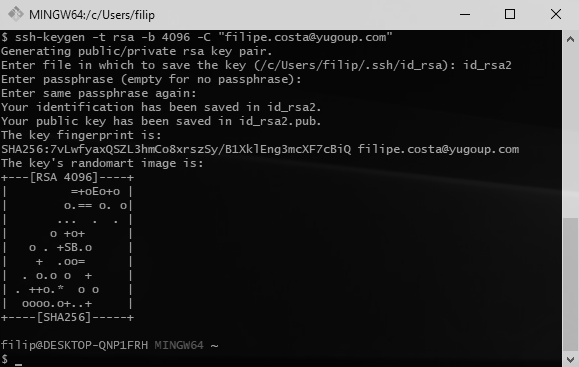
\includegraphics[width=0.6\linewidth]{Cap5/SSHKeyPairGeneration.png}
\caption{Consola de \textbf{Git Bash}}
\label{Fig:Fig10}
\end{figure}

\subsubsection{Comunicação via \textit{SSH}}

\hspace{1cm}Para ser adicionada a chave pública no \textbf{GitLab}, após serem acedidas as definições do utilizador, clica-se na opção \textit{SSH Keys} (\ref{Fig:Fig11}) e insere-se a chave pública -- o ficheiro com a terminação \textbf{.pub} -- que é um dos ficheiros gerados anteriormente. Pode optar-se também pela atribuição de um nome à chave e adição dessa chave ao conjunto de chaves. Depois de criado um par de chaves, é criado um novo repositório na interface web do \textbf{GitLab} que será clonado para a máquina.

\begin{figure}[hbt!]
\centering
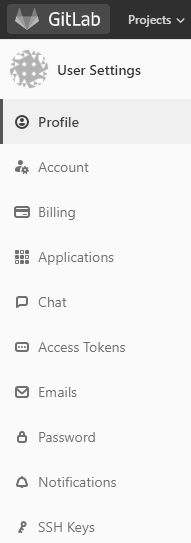
\includegraphics[width=0.2\linewidth]{Cap5/GitLabSettingsNavbar.png}
\caption{Menu de definições do utilizador do \textbf{GitLab}}
\label{Fig:Fig11}
\end{figure}

\hspace{1cm}Para clonar o repositório para a máquina é aberta a linha de comandos e executada a instrução \colorbox{gray}{\textcolor{white}{\$ git clone git@gitlab.com:nome\_utilizador/repositorio.git}}. De seguida seremos solicitados para inserir a password com a qual foi anteriormente criada a chave, ficando assim criada a pasta do projeto com ligação ao sistema de repositórios. A partir deste instante, todo o desenvolvimento da funcionalidade irá estar sincronizado entre o \textbf{GitLab} e o \textbf{Visual Studio} através do \textit{Team Explorer} que é uma ferramenta de integração de código desenvolvida e mantida pela equipa da \textbf{Microsoft} \cite{gitclone}.

\subsection{Desenvolvimento de testes unitários}

\hspace{1cm}Se o objetivo for desenvolver um \textit{package} seguindo a metodologia \textbf{TDD} o ideal será começar pela criação do projeto de teste. Como pode ser visto na figura \ref{Fig:Fig12}, terá de se alterar o nome do projeto para o nome pretendido.

\begin{figure}[hbt!]
\centering
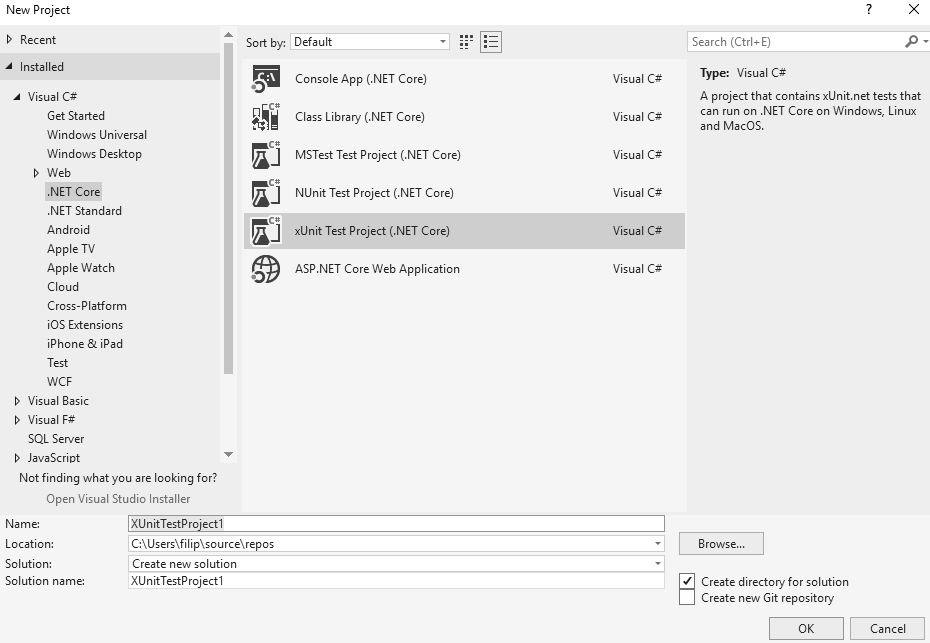
\includegraphics[width=0.7\linewidth]{Cap5/TestProjectCreation.png}
\caption{Menu de criação do projeto no \textit{Visual Studio 2017}}
\label{Fig:Fig12}
\end{figure}

\hspace{1cm}Após a criação do projeto de teste, são adicionados ao projeto os dois packages que são necessários para o desenvolvimento dos testes. São eles o \textbf{xUnit} e o \textbf{xUnit.runners.visualstudio} (\ref{Fig:Fig13}). 

\begin{figure}[hbt!]
\centering
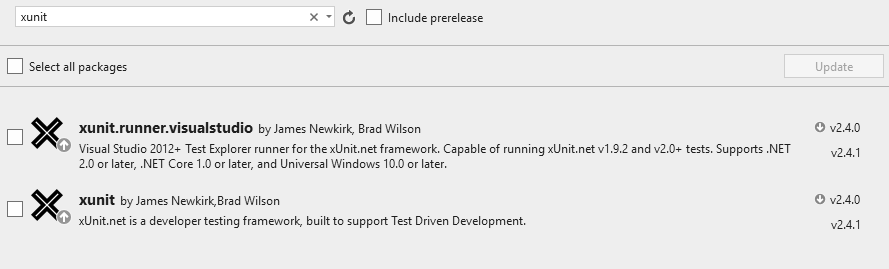
\includegraphics[width=0.7\linewidth]{Cap5/XUnitDependencies.png}
\caption{Biblioteca de \textit{packages} do \textit{Visual Studio 2017}}
\label{Fig:Fig13}
\end{figure}

\hspace{1cm}No desenvolvimento dos testes serão criados dois métodos. Um será utilizado para verificar se o resultado da soma é igual ao resultado esperado, outro para verificar se existe algum parâmetro com valor \textbf{null}.

\subsubsection{Criação da classe e estruturação dos métodos}

\hspace{1cm}Depois dos \textit{packages} estarem concluídos e -- antes de ser definida a classe como pública -- para começar o desenvolvimento da \textit{Theory}, é muito útil o apoio da documentação oficial que a \textbf{Microsoft} e a comunidade disponibilizam para se ter uma ideia mais consolidada sobre os métodos de desenvolvimento (\textbf{AAA}) de código para testes \cite{unittestingfundamentals}.
 
\subsubsection{\textit{Theory}}

\hspace{1cm}No contexto do desenvolvimento orientado a testes, a \textit{Theory} é, à semelhança dos atributos que vemos nos métodos de uma classe \textbf{controller}, um atributo que vai definir que tipo de testes serão desenvolvidos. Uma \textit{Theory} pode ser aplicada quando são desenvolvidos múltiplos casos de teste para o mesmo método. Se o objetivo for desenvolver apenas um caso de teste para um determinado método, deve ser utilizado o atributo \textit{Fact} \cite{unittestingxunit}.

\hspace{1cm}Adiciona-se uma classe para o desenvolvimento dos testes, \textit{UnitTestingInXUnit}, muda-se o nível de acesso para \textbf{public} e é iniciado o desenvolvimento da \textit{Theory} (\ref{Fig:Fig14}).

\begin{figure}[hbt!]
\centering
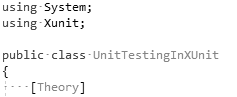
\includegraphics[width=0.4\linewidth]{Cap5/XUnitClass.png}
\caption{Classe \textit{UnitTestingInXUnit}}
\label{Fig:Fig14}
\end{figure}


\hspace{1cm}De seguida dá-se um nome, por exemplo \textit{shouldReturnASum}, ao método que é criado dentro da \textit{Theory} e passam-se três argumentos inteiros, \textbf{n1}, \textbf{n2} e \textbf{sum} (\ref{Fig:Fig15}).

\begin{figure}[hbt!]
\centering

\includegraphics[width=0.6\linewidth]{Cap5/TheoryMethod.png}
\caption{Método \textit{shouldReturnASum}}
\label{Fig:Fig15}
\end{figure}


\hspace{1cm}Dentro do método, é definida uma variável -- \textbf{sut} (\textit{system under test}) -- que é onde o sistema a ser testado estará contido. Uma vez que o objetivo é criar um método para calcular a soma de dois números, o sistema a ser testado -- \textbf{sut} -- será o objeto \textit{Calculator}.

\hspace{1cm}Esta será a fase de \textit{Arrange}. O \textbf{Visual Studio}, com a ajuda do \textit{intellisense}, permite-nos criar uma classe, num ficheiro novo, com o nome do objeto, a classe \textit{Calculator} e o método \textit{Add} (\ref{Fig:Fig16}).

\begin{figure}[hbt!]
\centering
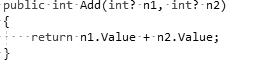
\includegraphics[width=0.4\linewidth]{Cap5/CalculatorClassAddMethod.png}
\caption{Método \textit{Add}}
\label{Fig:Fig16}
\end{figure}

\hspace{1cm}Após a criação da classe num ficheiro à parte, de volta ao projeto de teste, é iniciada a implementação da fase de \textit{Act}. Para esta fase é necessário definir outra variável chamada resultado que vai receber o resultado da soma dos dois números adicionados no método de adição. 

\hspace{1cm}Na implementação do teste, é invocado o método \textit{Add} na classe \textit{Calculator} para, só depois, se prosseguir para a fase de \textit{Assert} onde é verificado que o resultado obtido é igual ao esperado. A classe de teste deve ter sempre uma estrutura simples e organizada, com métodos à semelhança daquilo que pode ser visto na figura \ref{Fig:Fig17}. 

\begin{figure}[hbt!]
\centering
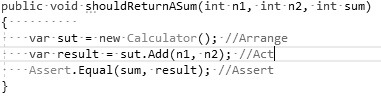
\includegraphics[width=0.5\linewidth]{Cap5/XUnitClassStructure.png}
\caption{Estrutura exemplo de um método}
\label{Fig:Fig17}
\end{figure}

\subsubsection{\textit{InlineData}}

\hspace{1cm}Para que a \textit{Theory} possa funcionar de forma correta, adiciona-se \textit{InlineData}. Estes atributos são colocados logo a seguir ao atributo \textit{Theory}. Começa-se pela adição de um caso de teste cujo resultado seja falso (e.g. 1 + 1 = 1) e outro caso de teste verdadeiro (e.g. 1 + 1 = 2) para ser feito um despiste e assim verificar-se que o método está a funcionar de acordo com o esperado (\ref{Fig:Fig18}).
 
 \begin{figure}[hbt!]
\centering
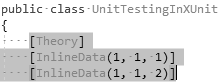
\includegraphics[width=0.3\linewidth]{Cap5/XUnitInlineData.png}
\caption{Atributos \textbf{[InlineData()]}}
\label{Fig:Fig18}
\end{figure}


\hspace{1cm}Como pode ser visto dentro do \textit{test explorer} (\ref{Fig:Fig19})
do ambiente integrado de desenvolvimento, um dos testes do método \textit{shouldReturnASum} passou e o outro teste falhou conforme esperado.

 \begin{figure}[hbt!]
\centering
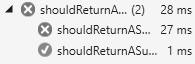
\includegraphics[width=0.3\linewidth]{Cap5/XUnitTestResults1.png}
\caption{Resultado da execução dos testes}
\label{Fig:Fig19}
\end{figure}

\hspace{1cm}Independentemente do número (\textbf{\textit{n}}) de testes que são executados, caso pelo menos um dos testes tenha resultado numa falha -- isto é caso a \textit{assertion} não se verifique -- a execução daquele método de teste (neste caso da \textit{Theory}) vai falhar completamente.

\hspace{1cm}A estrutura final da \textit{Theory}, para o caso de teste onde são adicionados dois números é relativamente simples. No entanto à medida que, para o mesmo caso, se aumenta o número cenários de teste em termos de \textit{InlineData}, aumenta também o nível de complexidade da \textit{Theory}. A \textit{Theory}, para todo o caso, ficará estruturada à semelhança daquilo que se pode ver na figura \ref{Fig:Fig20}.

 \begin{figure}[hbt!]
\centering
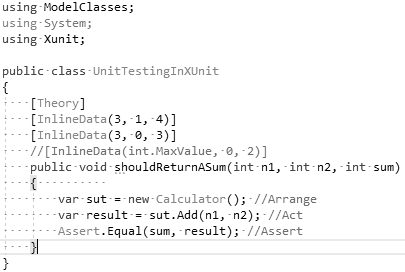
\includegraphics[width=0.5\linewidth]{Cap5/XUnitTestClassStructure2.png}
\caption{Estrutura completa de uma \textit{Theory}}
\label{Fig:Fig20}
\end{figure}

\subsubsection{Passagem de argumentos nulos}
\hspace{1cm}Pensemos no caso em que o utilizador passe um valor \textit{null} e espere que o método de adição faça \textit{output} a um resultado válido. Esta é uma validação que deve ser feita para dar seguimento à construção dos testes. Através da criação de um método de teste -- \textit{ShouldNotAddNULL} -- que simula este cenário, terá de se verificar que, caso exista um argumento \textit{null}, esse mesmo argumento será apanhado por uma exceção do tipo \textit{ArgumentNullException}.


\hspace{1cm}Para se validar que a classe \textbf{Calculator} lança uma exceção do tipo \textit{ArgumentNullException} quando algum dos dois parâmetros é nulo, é necessário em primeiro lugar adaptar a \textit{Theory} do método \textit{ShouldNotAddNULL} para que aceite valores inteiros que possam ou não existir. Para tal serão passados dois parâmetros do tipo ``\textit{int?}''. A seguir é iniciada uma instância do objeto \textbf{Calculator} -- que será o \textbf{sut} -- na fase de \textit{Arrange} para depois, nas fases de \textit{Act} e \textit{Assert} ser possível verificar que a excepção é lançada. Neste caso em particular, visível na figura \ref{Fig:Fig21}, foram agrupadas as fases de \textit{Act} e \textit{Assert} numa função \textbf{lambda}.

\begin{figure}[hbt!]
\centering
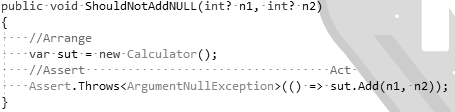
\includegraphics[width=0.6\linewidth]{Cap5/XUnitClass2.png}
\caption{Estrutura da segunda \textit{Theory}}
\label{Fig:Fig21}
\end{figure}

\hspace{1cm}Em segundo lugar, para se poderem passar números inteiros \textit{nullable}, terá de ser feita uma pequena alteração à classe \textbf{Calculator}. Em termos de estrutura, ficaria implementada -- dentro do método de adição -- uma condição (\textit{if}) que verificaria se os argumentos não são nulos. Caso exista algum argumento sem valor, é feito um \textit{throw} à exceção do tipo \textit{ArgumentNullException}. Caso contrário é retornado o resultado da soma dos dois valores (\ref{Fig:Fig22}). 

\begin{figure}[hbt!]
\centering
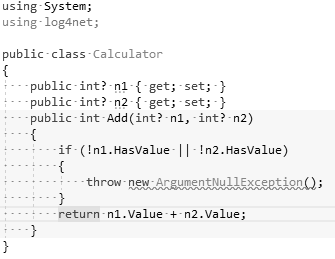
\includegraphics[width=0.5\linewidth]{Cap5/CalculatorNullArguments.png}
\caption{Estrutura da classe \textbf{Calculator} após alterações}
\label{Fig:Fig22}
\end{figure}

\hspace{1cm}De seguida, para validar que a \textit{Theory} executa os dois cenários de teste, são atribuidas duas linhas de \textit{InlineData()}. Por outras palavras, são criados dois casos de teste. O primeiro, que vai passar um valor nulo no lugar do primeiro argumento e o segundo que irá passar um valor nulo no lugar do segundo argumento. No final da adição destes casos de teste a \textit{Theory} terá aspeto semelhante ao da figura \ref{Fig:Fig23}.

\begin{figure}[hbt!]
\centering
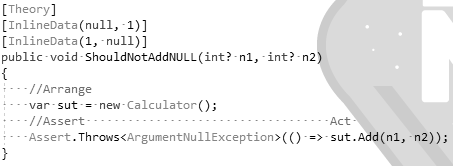
\includegraphics[width=0.5\linewidth]{Cap5/XUnitClass2Structure.png}
\caption{Estrutura da \textit{Theory} \textit{ShouldNotAddNULL} com os dois casos de teste}
\label{Fig:Fig23}
\end{figure}

\hspace{1cm}Nesta fase ambas as \textit{Theorys} estão devidamente desenvolvidas, com vários \textit{test cases}, com verificação e validação de funcionalidade. Por último lugar, para fechar a questão do desenvolvimento dos testes, são executados todos os testes para se verificar que passam como esperado (\ref{Fig:Fig24}). O código está pronto a ser publicado no sistema de repositórios.

\begin{figure}[hbt!]
\centering
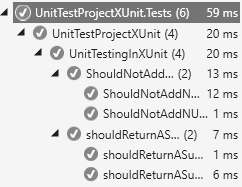
\includegraphics[width=0.4\linewidth]{Cap5/TestExplorerUnitTestingValidation.png}
\caption{Mostrador do \textit{Test Explorer}}
\label{Fig:Fig24}
\end{figure}

\subsection{Publicação do código no sistema de controlo de versões}

\hspace{1cm}No \textit{Team Explorer} podem ser publicadas as alterações feitas ao projeto, caso existam, clicando nas \textbf{Changes} (\ref{Fig:Fig25}). Depois terá de ser inserida uma mensagem que será publicada juntamente com o \textit{commit}. Nesta mensagem, é política da empresa colocar um \textit{briefing} dos ficheiros alterados, ou adicionados e, opcionalmente, pode ser especificada a funcionalidade adicionada. 

\begin{figure}[hbt!]
\centering
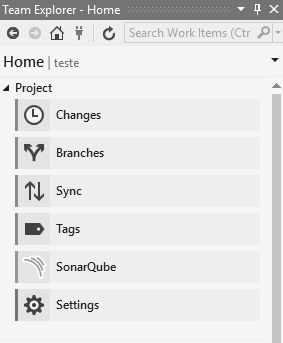
\includegraphics[width=0.4\linewidth]{Cap5/TeamExplorer.png}
\caption{Mostrador do \textit{Team Explorer}}
\label{Fig:Fig25}
\end{figure}

Clica-se em \textbf{Commit} e insere-se a password (\ref{Fig:Fig26}), gerada no momento da criação das chaves \textbf{SSH}, para que o código do projeto seja publicado no \textbf{VCS}.

\begin{figure}[hbt!]
\centering
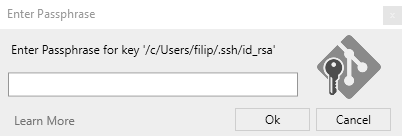
\includegraphics[width=0.5\linewidth]{Cap5/TeamExplorerSSHPassword.png}
\caption{Solicitador do \textbf{SSH}}
\label{Fig:Fig26}
\end{figure}

\hspace{1cm}Para a publicação do código deve ser utilizado um ficheiro que inclui ou exclui outro conjunto de ficheiros do projeto. Nem todos os ficheiros gerados são necessários para que o código possa ser executado. Alguns desses ficheiros são gerados automaticamente e não têm utilidade em termos de compilação. Portanto a inclusão ou exclusão deste conjunto de ficheiros -- através da utilização do \textbf{.gitignore} -- é indispensável para que numa fase mais avançada o código esteja compilável e seja reutilizável (https://github.com/github/gitignore). 

\subsection{Orquestração com \textit{Jenkins}}

\hspace{1cm}A configuração do \textbf{Jenkins} será feita na máquina de \textit{staging} disponibilizada pela empresa. A máquina está disposta em rede local. Isto torna o contacto com os dispositivos de visualização do estado das \textit{builds} mais facilitado. Mais à frente este tema é devidamente abordado.

\subsubsection{Instalação dos plugins}

\hspace{1cm}Para que possam ser executadas as \textit{builds} da compilação de código do módulo de soma, juntamente com os respetivos testes unitários e a análise estática, é necessária a instalação de um conjunto de \textit{Plugins} no \textbf{Jenkins}, nomeadamente:

\begin{itemize}
 \item Credentials;
 \item MSBuild Plugin;
 \item Gitlab Plugin;
 \item Blue Ocean (opcional);
 \item Slack Notification (opcional);
\end{itemize}

Da lista acima é obrigatório o uso dos \textit{plugins} \textbf{Credentials}, \textbf{MSBuild} e \textbf{Gitlab}, utilizados para compilação de código do projeto C\#. O \textbf{Credentials} faz a gestão das credenciais de acesso ao repositório do sistema de controlo de versões sem que estas sejam expostas. O \textbf{MSBuild} é a plataforma utilizada para fazer \textit{build} de projetos \textbf{.NET}. O \textbf{Gitlab} é utilizado para estabelecer uma ligação segura ao \textbf{VCS}. Os restantes \textit{plugins} são opcionais dado que o \textbf{Blue Ocean} é uma interface de visualização do \textbf{Jenkins} que apenas apresenta uma interface gráfica mais apelativa para o utilizador. Já o \textbf{Slack Notification} é um componente adicional para o sistema de visualização, caso se pretenda que os \textit{developers} recebam notificações no \textit{Slack} -- canal de comunicação utilizado pela empresa -- sobre os diferentes acontecimentos durante as fases da \textit{pipeline}.

\subsubsection{Instalação dos módulos de desenvolvimento do C\#}

\hspace{1cm}Será necessário descarregar o \textbf{.NET Core SDK}, que já inclui o \textbf{.NET Core Runtime}, tendo sempre em mente o sistema operativo que é utilizado. Neste caso é utilizado o \textbf{Windows 10}. Estes componentes podem ser descarregados a partir do site oficial da \textbf{Microsoft}.

Com o \textit{Software Development Kit} (SDK) devidamente instalado, neste caso na máquina de \textit{staging}, procede-se à configuração do \textbf{Jenkins}. Como dito anteriormente, esta ferramenta de integração contínua fará \textit{fetch} ao código presente no sistema de controlo de versões via \textbf{SSH} para depois poderem ser feitas operações sobre o mesmo. Para que tal seja possível, providencia-se ao orquestrador de processos a chave pública para que possa comunicar com o \textbf{GitLab} e é indicado, nas opções de configuração do \textbf{Jenkins}, o caminho da localização do \textbf{MSBuild} instalado anteriormente na máquina.

\subsubsection{Configuração das credenciais de acesso ao GitLab}

\hspace{1cm}Com o \textit{plugin} de gestão de credenciais (\textbf{Credentials}) instalado, é adicionada uma nova credencial de acesso. Para tal, clica-se em cima do \textit{plugin} \textbf{Credentials} e acede-se à opção que foi expandida, ``System'' (\ref{Fig:Fig28}).

\begin{figure}[hbt!]
\centering
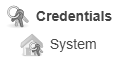
\includegraphics[width=0.15\linewidth]{Cap5/JenkinsCredentials.png}
\caption{\textit{Plugin} \textbf{Credentials}}
\label{Fig:Fig28}
\end{figure}

\hspace{1cm}De seguida clica-se em \textit{Global credentials} e adiciona-se uma nova credencial (\textit{Add Credentials}). Depois, seleciona-se o tipo de credencial na \textit{dropdownlist} como ``SSH Username with private key'' e insere-se diretamente a chave privada, selecionando a opção ``Enter directly'', no campo ``Private Key'', como pode ser visto na figura \ref{Fig:Fig29}.

\begin{figure}[hbt!]
\centering
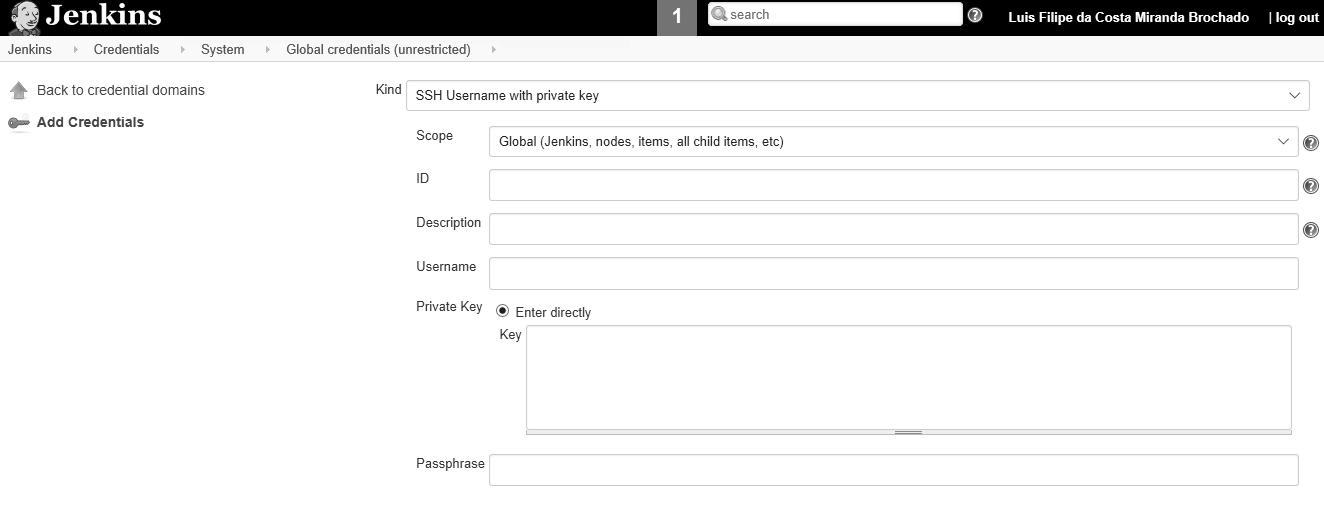
\includegraphics[width=0.9\linewidth]{Cap5/JenkinsCredentialsConfig.png}
\caption{Configuração das credenciais de acesso}
\label{Fig:Fig29}
\end{figure}

\subsubsection{Configuração do \textbf{MSBuild}}

\hspace{1cm}Nas opções de configuração do \textbf{Jenkins}, em \textbf{Manage Jenkins}, existe um conjunto de opções à disposição. Será selecionada a opção \textbf{Global Tool Configuration}. Se o \textit{plugin} \textbf{MSBuild} tiver sido instalado, deverá aparecer nas opções de instalação uma imagem semelhante à da figura \ref{Fig:Fig30}. 

\begin{figure}[hbt!]
\centering
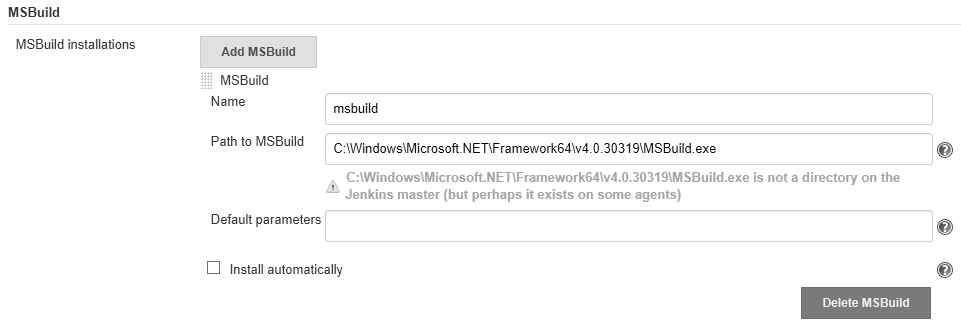
\includegraphics[width=0.9\linewidth]{Cap5/JenkinsGlobalToolConfiguration.png}
\caption{Caminho de instalação do \textbf{MSBuild}}
\label{Fig:Fig30}
\end{figure}

\hspace{1cm}Com o caminho absoluto do ficheiro executável do \textbf{MSBuild} colocado na opção ``Path to MSBuild'', o orquestrador de processos está pronto a compilar o código dos projetos \textbf{.NET}. Nesta fase a configuração do orquestrador está concluída. De seguida será abordada a configuração da \textit{pipeline} testes automatizados.

\subsection{Configuração da \textit{pipeline}}

\hspace{1cm}Começando pela criação de um \textit{New Item}, é atribuído um nome à escolha do utilizador selecionando a opção \textit{Freestyle project}. O primeiro \textit{job} está criado e segue-se sua configuração. Este \textit{job} será o primeiro componente da \textit{pipeline}.

\subsubsection{Estrutura dos \textit{jobs}}

\hspace{1cm}Para a configuração começa-se por dar uma descrição ao \textit{job} e por selecionar a opção para descartar builds anteriores -- ``Discard old build'' -- para que sejam eliminados todos os ficheiros e artefactos resultantes de compilações de código anteriores. Depois adiciona-se o \textbf{GitLab Plugin} à lista de \textit{plugins} para que seja possível configurar uma ligação ao \textbf{VCS} através da criação de um \textbf{API token}. Para configurar esta ligação é necessário aceder novamente às propriedades de configuração do sistema -- \textbf{Configure System} -- e navegar até aparecer a secção de configuração do \textbf{GitLab} (\ref{Fig:Fig31}).

\begin{figure}[hbt!]
\centering
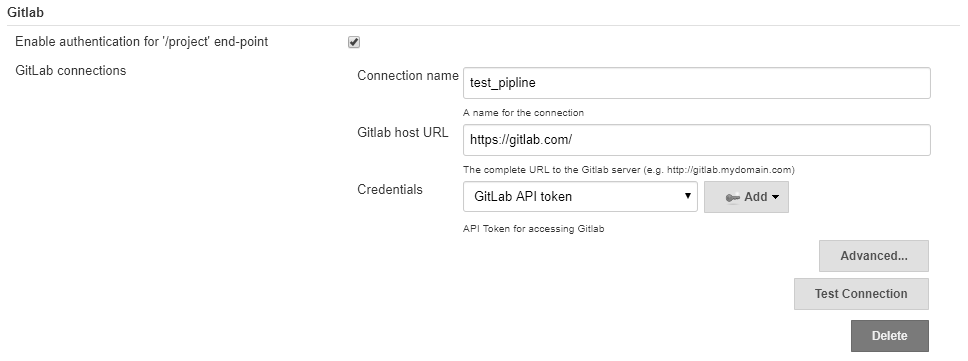
\includegraphics[width=0.9\linewidth]{Cap5/ConfigureSystem.png}
\caption{Configuração da ligação ao \textbf{GitLab}}
\label{Fig:Fig31}
\end{figure}

\hspace{1cm}Antes de ser adicionado um \textit{Access Token} ao orquestrador de processos é necessário requisitar, dentro do sistema de controlo de versões, um novo \textit{Personal Access Token}. Para tal, acede-se à plataforma \textbf{GitLab}, navega-se até aos \textit{user settings}, clica-se em \textit{Access Tokens} e adiciona-se um nome, uma data de validade e os \textbf{scopes} do \textit{token} como mostrado na figura \ref{Fig:Fig32}.

\begin{figure}[hbt!]
\centering
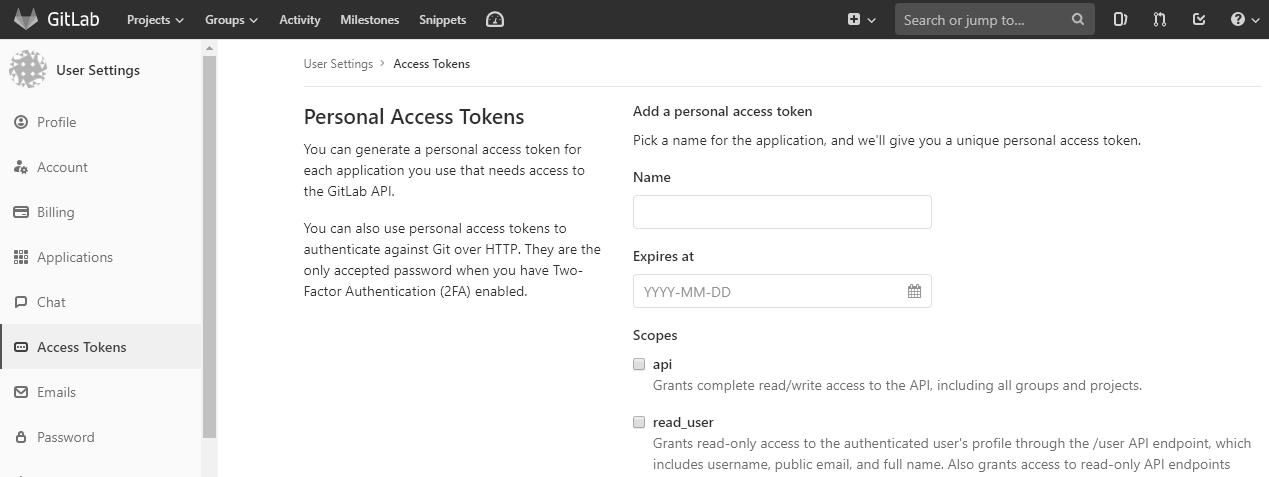
\includegraphics[width=0.9\linewidth]{Cap5/GitLabAccessToken.png}
\caption{Menu de criação do \textit{Personal Access Token} }
\label{Fig:Fig32}
\end{figure}

O \textit{access token} criado será depois adicionado nas credenciais do \textbf{Jenkins}. Este \textit{access token} só pode ser visualizado uma única vez por questões de segurança e, por boa prática, não deve ser utilizado em mais que um serviço.

\hspace{1cm}Voltando à configuração do \textit{job}, com a \textit{GitLab Connection} configurada, seguem-se as configurações de \textbf{Source Code Management}. É aqui que serão configuradas a ligações via \textbf{SSH} aos respetivos repositórios criados que foram armazenados no \textbf{VCS}. Assim sendo seleciona-se a opção \textbf{Git} e preenche-se o \textbf{URL} do repositório com a hiperligação do protocolo \textbf{SSH}, com as respetivas credenciais de acesso, que é o meio de ligação pretendido para estabelecer a conexão. A \textit{branch} que será utilizada para fazer \textit{build} é a única existente no projeto (\ref{Fig:Fig33}), \textbf{master}.

\begin{figure}[hbt!]
\centering
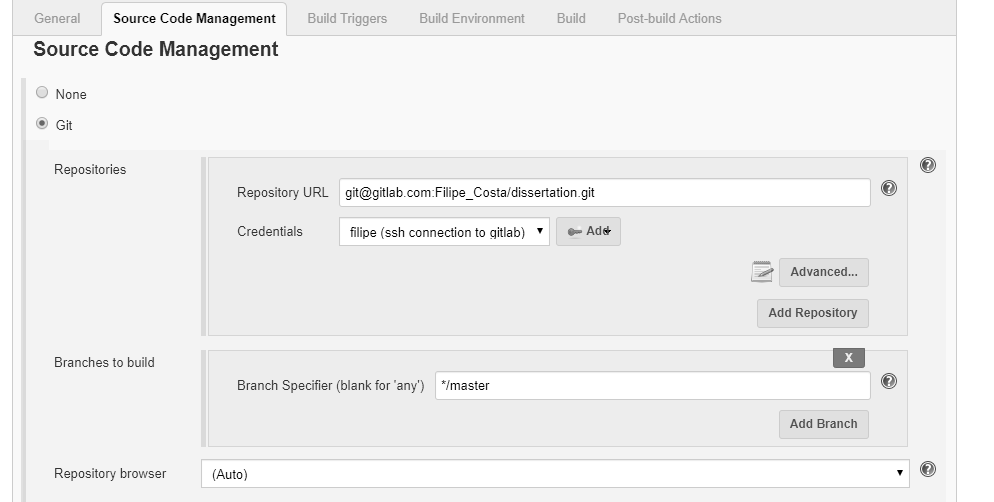
\includegraphics[width=0.9\linewidth]{Cap5/JenkinsSourceCodeManagement.png}
\caption{\textit{Source Code Management}}
\label{Fig:Fig33}
\end{figure}

\hspace{1cm}O próximo separador, \textbf{Build Triggers}, vai ser passado à frente uma vez que não é necessário qualquer tipo de configuração neste campo. Este segmento -- \textbf{Build Triggers} -- é onde são agendados \textit{triggers} automáticos a novas \textit{builds} mediante certos eventos. Será utilizado mais à frente, por exemplo, na configuração dos \textit{jobs} que serão dependentes da execução deste primeiro \textit{job}.

\hspace{1cm}No próximo segmento, \textbf{Build Environment}, é selecionada a opção ``Delete workspace before build starts''. Esta opção, segundo a tradução literal do Inglês, significa que é apagado o \textit{worskpace} gerado pelo \textbf{Jenkins} sempre que começar uma \textit{build} (\ref{Fig:Fig34}). 

\begin{figure}[hbt!]
\centering
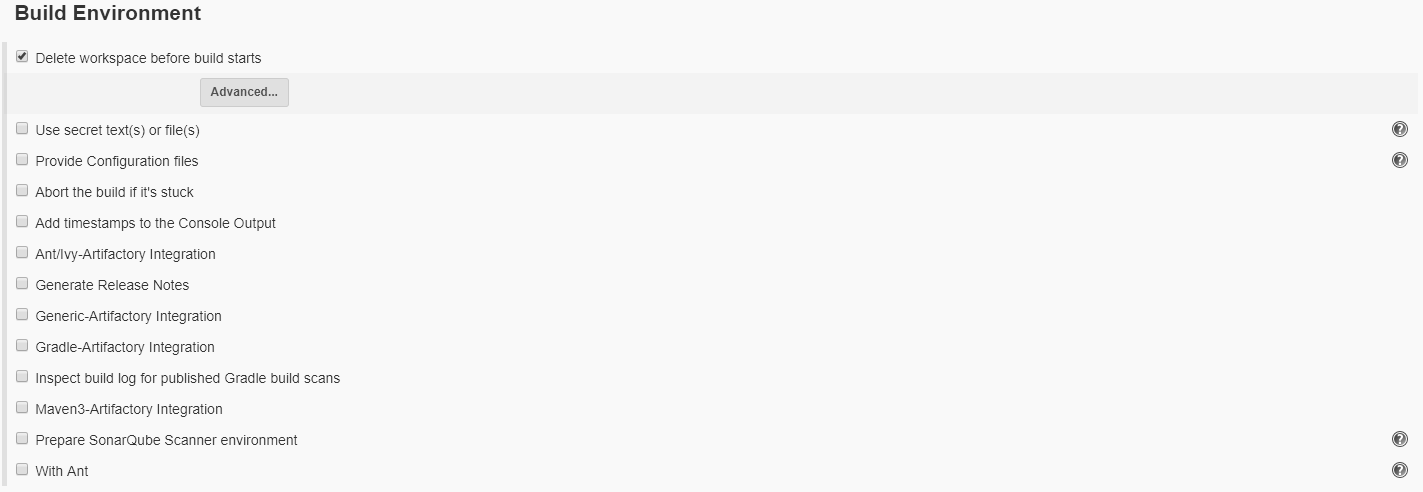
\includegraphics[width=0.9\linewidth]{Cap5/JenkinsBuildEnvironment.png}
\caption{\textit{Build Environment}}
\label{Fig:Fig34}
\end{figure}

Esta funcionalidade tem como objetivo evitar que execuções anteriores da \textit{pipeline} provoquem erros devido a versões de serviços e/ou dependências antigas que tenham sido usados e não tenham sido atualizados corretamente para a nova execução.

\subsection{Integração dos serviços}

\hspace{1cm}Para a integração de serviços externos na \textit{pipeline} vão ser utilizados:

\begin{itemize}
 \item \textbf{Docker};
 \item \textbf{SonarQube};
 \item \textbf{Nexus Repository Manager OSS 2};
 \item \textbf{Docker Registry 2.0};
\end{itemize}

\hspace{1cm}Na fase de \textit{\textbf{Build}}, vão ser inseridas as instruções que normalmente seriam introduzidas numa linha de comandos. Para que estejamos mais contextualizados com as instruções que são utilizadas aconselha-se a consulta da documentação oficial de apoio da \textbf{Microsoft} referente ao \textbf{.NET Core CLI} \cite{dotnetcorecli}. Toda a informação que é necessária está disponível nesta documentação.

\subsubsection{Integração com \textbf{SonarQube}}

\hspace{1cm}Comecemos por integrar a análise estática na \textit{pipeline}. Para fazer a análise estática do código é utilizada uma \textit{tool} de revisão de código chamada \textbf{SonarQube}. Esta ferramenta de análise estática já integra com \textbf{Docker} portanto vai ser executada uma instância de uma versão do \textbf{SonarQube} dentro de um \textit{container} que será publicado na porta 9000. Todos os dados serão guardados dentro de um \textit{container} do \textbf{Docker} que foi anteriormente criado através de uma técnica de persistência de dados em volume \cite{dockervolumes}. Desta forma, sempre que for necessário, os dados podem ser acedidos através do \textit{attachment} de um \textit{container} a este volume de dados conferindo assim a possibilidade e a garantia de se utilizar uma instância para aceder às informações guardados sobre os projetos. 

\hspace{1cm}A configuração de um projeto dentro da instância do \textbf{SonarQube} é relativamente simples. As credenciais de autenticação, por defeito, são \colorbox{gray}{\textcolor{white}{admin}} para o \textbf{username} e \colorbox{gray}{\textcolor{white}{admin}} para \textbf{password}. Todos os projetos são criados da mesma forma, independentemente da linguagem utilizada. Neste caso é selecionada a opção ``criar novo projeto'' e, após a atribuição de uma chave e de um nome ao projeto, adiciona-se um \textit{token} de identificação. De seguida é selecionada a linguagem em que o projeto foi desenvolvido. É importante ter em consideração que tanto a atribuição do \textit{token} como a seleção da linguagem em que o projeto foi desenvolvido são dois passos que também têm relevância para a integração do \textbf{SonarQube} com a \textit{pipeline}. Mais tarde será necessário a chave que atribuída ao projeto nesta fase. 

\hspace{1cm}A instrução que se vai utilizar para dar início à análise estática é a seguinte: \colorbox{gray}{\textcolor{white}{\$ dotnet SonarScanner.MSBuild.dll begin /k:``project-key''}} e caso se pretenda, por exemplo, executar a análise estática a partir de um \textit{container} dentro de uma máquina virtual, podem ser adicionadas como opções \colorbox{gray}{\textcolor{white}{/d:sonar.host.url=``hostname''}} para indicar o \textit{hostname} onde será feita análise e \colorbox{gray}{\textcolor{white}{/d:sonar.login=``access\_token''}} para indicar o \textit{access token} que permite aceder ao \textit{container}. É necessário ter em conta que o \textbf{Jenkins} não reconhece nem o comando \textit{dotnet}, nem a ``.dll'' do \textit{SonarScanner}, portanto são necessários os \textit{absolute paths} destes dois ficheiros dentro da máquina principal para que o orquestrador os consiga encontrar (\ref{Fig:Fig35}).

\begin{figure}[hbt!]
\centering
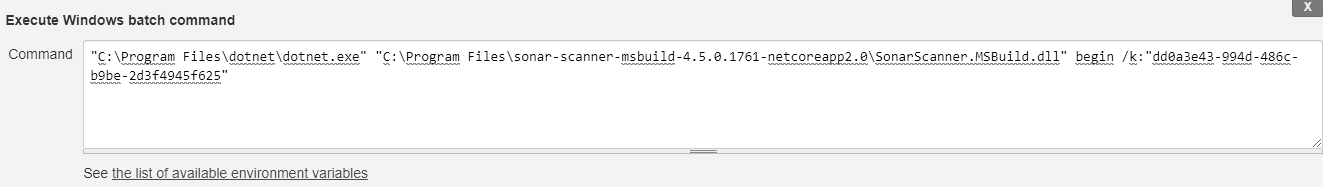
\includegraphics[width=0.9\linewidth]{Cap5/JenkinsSonarQubeStart.png}
\caption{Primeira instrução do \textbf{SonarQube}}
\label{Fig:Fig35}
\end{figure}

\hspace{1cm}Para concluir a análise estática é necessário utilizar como última instrução: \colorbox{gray}{\textcolor{white}{\$ dotnet SonarScanner.MSBuild.dll end}} (\ref{Fig:Fig36}). No caso em que a análise estática é iniciada com as opções extra, é necessário executar a instrução descrita neste parágrafo com a adição da opção \colorbox{gray}{\textcolor{white}{/d:sonar.login=``access\_token''}} para encerrar corretmente a execução da análise estática.

\begin{figure}[hbt!]
\centering
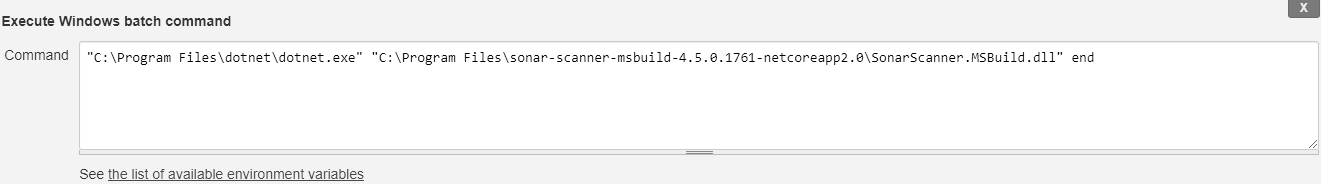
\includegraphics[width=0.9\linewidth]{Cap5/JenkinsSonarQubeFinish.png}
\caption{Última instrução do \textbf{SonarQube}}
\label{Fig:Fig36}
\end{figure}

\hspace{1cm}Executa-se a instrução para iniciar a ferramenta de análise estática no início do \textit{job} para que -- durante as fases de \textit{build} e \textit{testing} -- todo o código da aplicação seja revisto. É executada a instrução para terminar a ferramenta antes do final do \textit{job} para que seja parada a execução desta \textit{tool} \cite{sonarqubejenkins}. Os resultados da análise estática serão apresentados à semelhança daquilo que se pode ser visto na figura \ref{Fig:Fig37}.

\begin{figure}[hbt!]
\centering
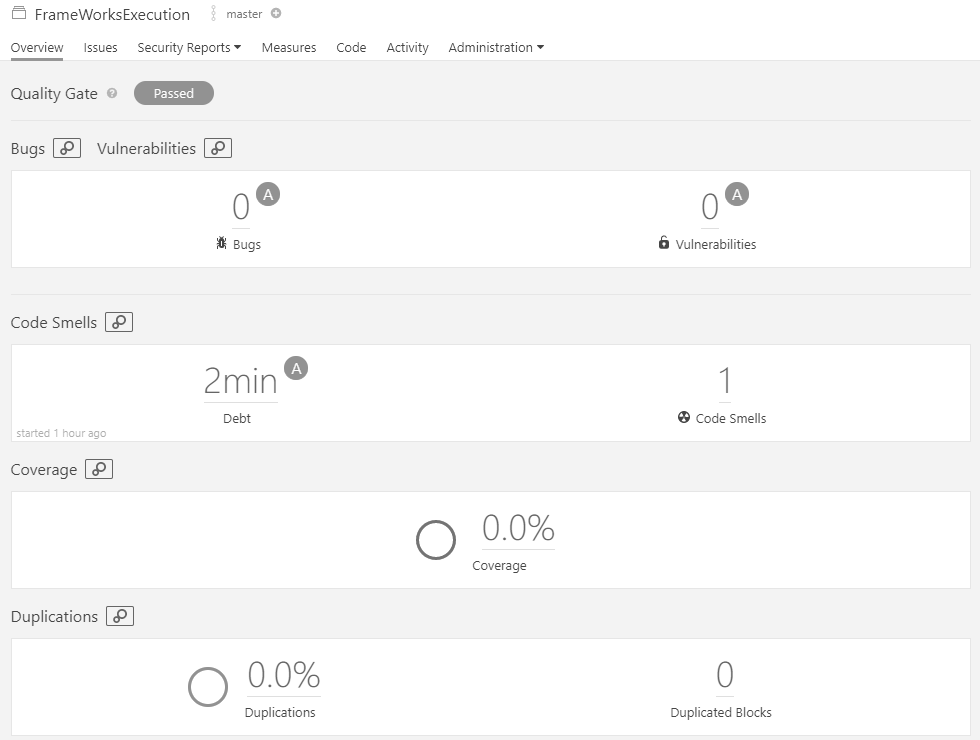
\includegraphics[width=0.8\linewidth]{Cap5/SonarQube.png}
\caption{SonarQube -- Quality Gate}
\label{Fig:Fig37}
\end{figure}

\subsubsection{\textit{Build} do projeto e dos testes}

\hspace{1cm}Para se fazer \textit{build} a um projeto (.csproj) ou a uma solução (.sln) a instrução é: \colorbox{gray}{\textcolor{white}{\$ dotnet build project-path}} \cite{dotnetbuild}. Aqui entramos na fase de \textit{build} (\ref{Fig:Fig38}) do projeto e dos testes unitários que foram criados para a aplicação calculadora.

\begin{figure}[hbt!]
\centering
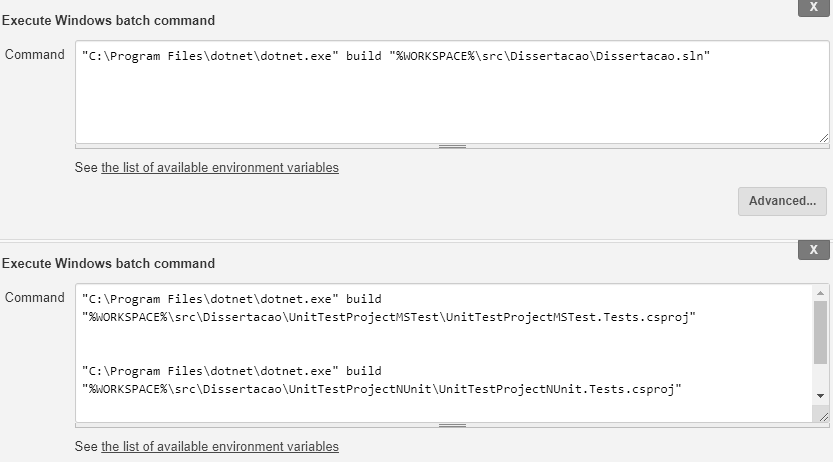
\includegraphics[width=0.9\linewidth]{Cap5/JenkinsProjectBuild.png}
\caption{Instruções de \textit{build} dos projetos}
\label{Fig:Fig38}
\end{figure}

\hspace{1cm}Após a fase de \textit{build}, são executados os testes para o \textbf{Jenkins} interpretar os seus resultados e produzir um gráfico com a estatística dos \textit{test runs}. A instrução utilizada para produzir os resultados dos testes em formato interpretável (.trx) foi a seguinte: \colorbox{gray}{\textcolor{white}{\$ dotnet test project-path -{}-no-build -{}-logger trx}} \cite{dotnettest}.\\ Esta instrução produz um ficheiro (.trx) com o resultado dos testes que é interpretado pelo orquestrador e apresentado na GUI (\ref{Fig:Fig39}). 

\begin{figure}[hbt!]
\centering
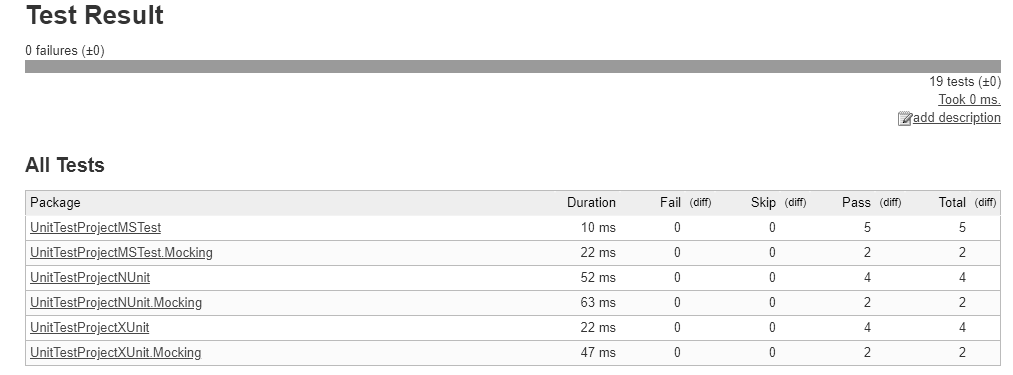
\includegraphics[width=0.9\linewidth]{Cap5/JenkinsTestResult.png}
\caption{Resultado dos testes unitários}
\label{Fig:Fig39}
\end{figure}

\subsubsection{Integração com o repositório \textit{Nexus Repository Manager OSS}}

\hspace{1cm}A ferramenta de armazenamento de artefactos utilizada é o \textbf{Nexus Repository Manager OSS}. Este sistema de gestão de artefactos tem integração com \textbf{Docker} -- que foi o motivo com mais peso na sua seleção -- e apresenta uma \textbf{GUI} de simples utilização. Para a \textit{pipeline} foi escolhida uma versão mais antiga, a versão \textbf{2.14.12-02}, uma vez que durante a escrita do documento cumpria com os requisitos estabelecidos pela orientação. A versão \textbf{2.14.13-01} também pode ser utilizada uma vez que não existem diferenças tanto em termos de utilização como de configuração.

\hspace{1cm}Para que seja possível publicar artefactos dentro de um \textit{container} com uma instância do \textbf{Nexus} é necessário realizar um conjunto de operações. Por outras palavras, é preciso empacotar o módulo de soma, \textit{ModelClasses}, para um formato específico e assim transformar o módulo de soma de dois números inteiros num \textbf{NuGet Package}. Esta operação pode ser feita através da utilização da instrução: \colorbox{gray}{\textcolor{white}{\$ dotnet pack project-path}} \cite{dotnetpack}. Esta instrução gera um ficheiro do tipo ``\textbf{.nupkg}'' que é o módulo \textit{plug-and-play} da funcionalidade desenvolvida.

\hspace{1cm}O próximo passo é a configuração do repositório. Para configurar corretamente o repositório aconselha-se a leitura da documentação produzida pela \textbf{Sonatype} \textbf{\cite{sonatypenexus}} e disponibilizada no repositório público de imagens do \textbf{Docker} \textbf{\cite{sonatypenexusdocker}}. A configuração do repositório \textbf{NuGet} requer a criação de dois repositórios, um \textit{proxy} e um \textit{hosted}, que mais tarde vão ser colocados dentro de um grupo, \textit{public}, resultando no total de três repositórios criados. As credenciais de autenticação por defeito são \colorbox{gray}{\textcolor{white}{admin}} para o \textbf{username} e \colorbox{gray}{\textcolor{white}{admin123}} para \textbf{password}. A criação dos repositórios do \textbf{Nexus} é ligeiramente mais complexa em termos processuais e, comparativamente com a configuração do \textbf{SonarQube}, requer alguns cuidados. Por defeito, o \textbf{Nexus} traz consigo um conjunto de repositórios \textbf{Maven} pré-configurados que podem ser eliminados. 

\hspace{1cm}Começando pela adição de um repositório \textit{proxy}, é atribuido o ID ``nuget-gallery-proxy'' e o nome ``Nuget Gallery Proxy''. Como pode ser visto na figura \ref{Fig:Fig40}, no campo \textit{Provider} seleciona-se \textbf{NuGet} como formato do artefacto e coloca-se a conexão à \textbf{API} pública do \textbf{NuGet} no campo \textit{Remote Storage Location}.

\begin{figure}[hbt!]
\centering
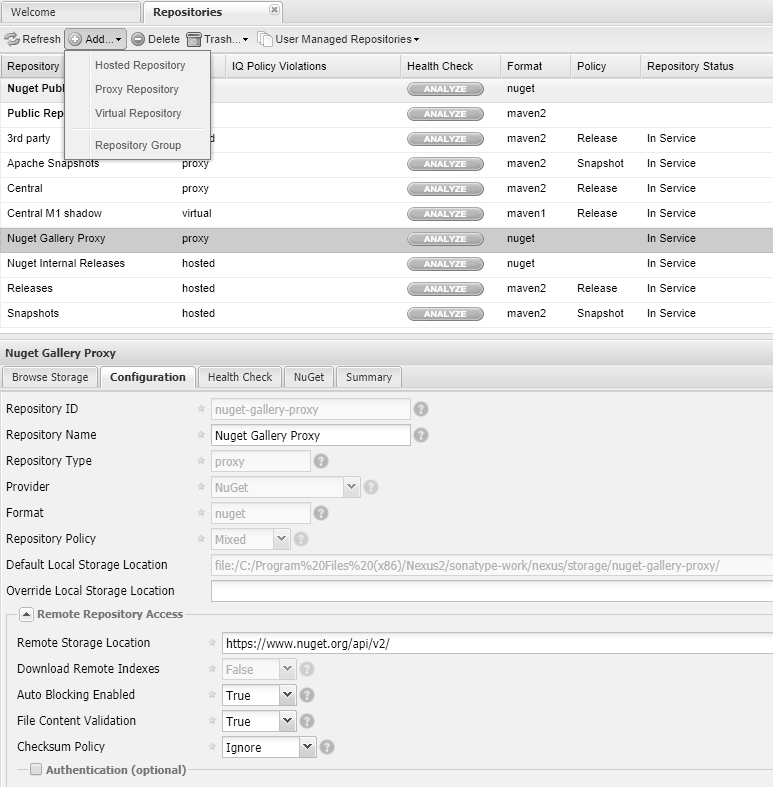
\includegraphics[width=0.9\linewidth]{Cap5/NexusOSSProxy.png}
\caption{Configuração do repositório NuGet proxy}
\label{Fig:Fig40}
\end{figure}

\hspace{1cm}De seguida cria-se o repositório \textit{hosted}, atribuindo como ID ``nuget-releases'' e como nome ``Nuget Internal Releases''. À semelhança da configuração anterior, o \textit{Provider} é o mesmo, ou seja, \textit{NuGet}. Nas definições de acesso podem ser selecionadas as opções \textit{Allow Redeploy} ou \textit{Disable Redeploy} consoante se pretenda ou não permitir \textit{overwriting} a pacotes de versões semelhantes. Para testar o repositório aconselha-se a \textit{Policy} de \textit{Allow Redeploy} uma vez que não bloqueia a entrada a \textbf{NuGet packages} da mesma versão sendo mais fácil de verificar o seu funcionamento.

\hspace{1cm}Por último, o grupo que vai conter os dois repositórios. Para configurar o grupo de repositórios no \textbf{Nexus} são apenas necessários um ID, por exemplo ``nuget-public'', e um nome semelhante, ``Nuget Public''. De seguida, passam-se os repositórios \textit{hosted} e \textit{proxy} -- presentes nos \textit{Available Repositories} -- para os \textit{Ordered Group Repositories} (\ref{Fig:Fig41}). 

\begin{figure}[hbt!]
\centering
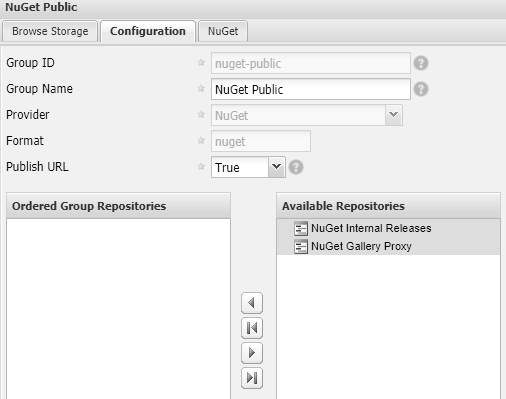
\includegraphics[width=0.9\linewidth]{Cap5/NexusPublic.png}
\caption{Configuração do repositório NuGet Public}
\label{Fig:Fig41}
\end{figure}

\hspace{1cm}A configuração do repositório de \textbf{NuGet packages} está praticamente concluída. Para publicar \textbf{Packages} no repositório é necessário aceder à API Key gerada pelo \textbf{Nexus}. Para tal, vai-se ao painel de administração na opção \textit{server} e, nas \textit{security settings}, coloca-se a \textit{NuGet API-Key Realm} nos \textbf{Selected Realms} (\ref{Fig:Fig42}).

\begin{figure}[hbt!]
\centering
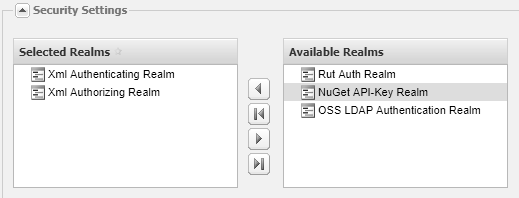
\includegraphics[width=0.9\linewidth]{Cap5/NexusSecurity.png}
\caption{Configurações de segurança do servidor Nexus}
\label{Fig:Fig42}
\end{figure}

\hspace{1cm}A \textbf{Sonatype} disponibiliza no seu canal oficial de \textbf{Youtube} um vídeo mais detalhado sobre a gestão de componentes .NET com o \textbf{Nexus} \cite{managingdotnetcomponentswithnexus}. A última instrução da fase de \textit{build} vai colocar o \textit{package} no repositório que foi configurado. Esta instrução necessita da \textbf{API Key} para autenticar contra o repositório do \textbf{Nexus}, precisa também da hiperligação (\textit{source}) para onde será enviado o pacote e precisa do caminho absoluto do ficheiro produzido com a instrução anterior. Pode utilizar-se uma instrução semelhante à seguinte:  \colorbox{gray}{\textcolor{white}{dotnet nuget push}}, com o caminho do \textit{package} \colorbox{gray}{\textcolor{white}{package-path}}, com a \textbf{API Key} \colorbox{gray}{\textcolor{white}{-k nexus-api-key}} e com a \textit{source} \colorbox{gray}{\textcolor{white}{-s hosted-repository}} como opções \cite{dotnetnuget}.

\begin{figure}[hbt!]
\centering
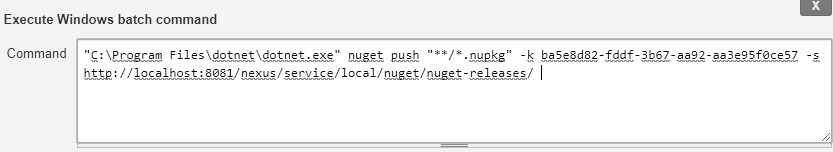
\includegraphics[width=0.9\linewidth]{Cap5/JenkinsPushToNexus.png}
\caption{Instrução de publicação do \textit{package} para o Nexus}
\label{Fig:Fig43}
\end{figure}

\hspace{1cm}A instrução é semelhante aquela visível na figura \ref{Fig:Fig43} sendo que se pode recorrer a \textit{wildcards} (*) para procurar ficheiros pelo seu formato. Está tudo configurado para se fazer \textit{build} do primeiro \textit{job} da \textit{pipeline}. O próximo passo é o desenvolvimento de uma \textbf{Web API} que implemente a funcionalidade de soma.

\subsection{Desenvolvimento da Web API}

\hspace{1cm}Para o desenvolvimento da \textbf{Web API} será utilizada uma ferramenta de documentação, o \textbf{Swagger} \cite{aboutswagger}. Esta ferramenta \textit{open source} é utilizada pela comunidade de \textit{developers} principalmente no desenvolvimento de \textbf{APIs REST}.

\hspace{1cm}Como dito anteriormente, será utilizado o \textbf{NuGet package} -- \textit{ModelClasses} -- e são também necessárias algumas alterações ao código, nomeadamente a adição do serviço de documentação do \textbf{Swagger} na classe \textit{Startup.cs}. O serviço que se vai desenvolver não incorpora uma base de dados uma vez que para testar os serviços em funcionamento não seria necessário armazenar dados da \textbf{Web API} nesta fase de desenvolvimento. 

\hspace{1cm}Depois do desenvolvimento da API, ainda dentro da mesma solução, será criado um projeto de teste onde vão ser desenvolvidos os testes de integração e performance aos \textit{endpoints} disponíveis.

\subsubsection{Pré-requisitos:}

\begin{itemize}
 \item Swashbuckle.AspNetCore (4.0.1);
 \item Swashbuckle.AspNetCore.Swagger (4.0.1);
 \item ModelClasses (1.0.3.4);
 \item Microsoft.AspNetCore.App;
 \item Microsoft.AspNetCore.App.Design;
\end{itemize}

\subsubsection{Configuração da nova \textit{source} no \textit{Visual Studio}}

\hspace{1cm}Para ser adicionada a nova \textit{source} no \textbf{Visual Studio} é necessário aceder a \textit{``Tools''} e clicar em \textit{``options''}. Depois navega-se novamente até se encontrarem as definições de configuração do \textit{``NuGet Package Manager''} e adiciona-se a nova fonte na opção \textit{``Package Sources''} para que possam ser incluídos no projeto os pacotes com as dependências necessárias (\ref{Fig:Fig44}).

\begin{figure}[hbt!]
\centering
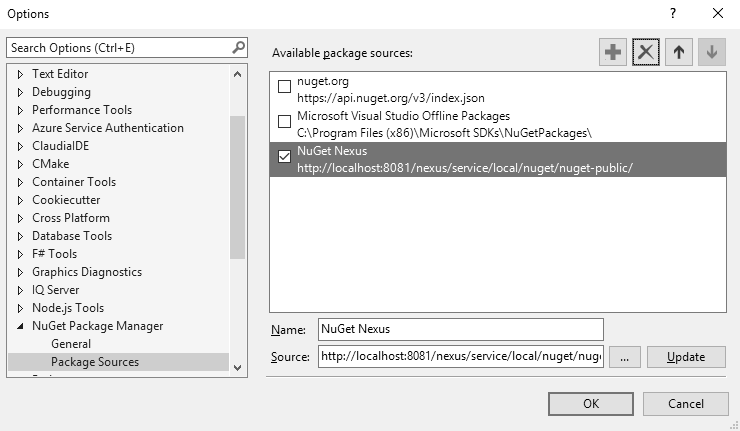
\includegraphics[width=0.7\linewidth]{Cap5/VSPackageSource.png}
\caption{NuGet Package Manager}
\label{Fig:Fig44}
\end{figure}

Todos os pacotes estão incluídos na nova \textit{source}, mesmo aqueles que são disponibilizados na API do \textbf{NuGet} (https://www.nuget.org/api/v2), porque o repositório \textit{proxy} foi configurado para incluir a API pública de \textbf{NuGet Packages}.

\subsubsection{Alterações ao serviço da Web API}

\hspace{1cm}No serviço, começa-se por editar a classe ``Startup.cs'' para incluir a interface do \textbf{Swagger}. Em primeiro lugar são incluídos os \textit{packages} do \textbf{Swashbuckle} nas dependências e, de seguida, dentro da classe incluem-se os serviços do \textbf{Swagger} nos métodos de configuração do serviço (\ref{Fig:Fig45}) e da aplicação especificada (\ref{Fig:Fig46}). A configuração do \textbf{Swagger} está, uma vez mais, em detalhe na documentação oficial \cite{dotnetwithswagger} do .NET pelo que se aconselha a sua leitura.

\begin{figure}[hbt!]
\centering
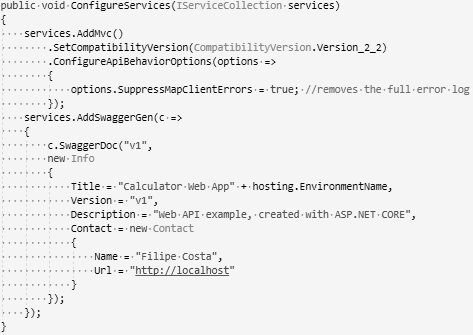
\includegraphics[width=0.65\linewidth]{Cap5/VSStartupClass1.png}
\caption{Estrutura do método de configuração do serviço}
\label{Fig:Fig45}
\end{figure}

\begin{figure}[hbt!]
\centering
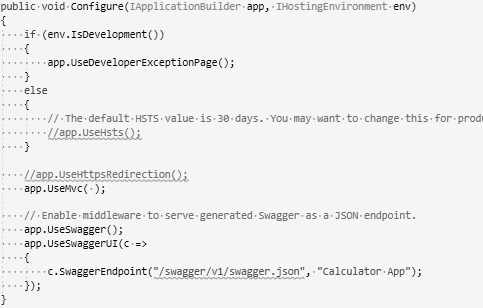
\includegraphics[width=0.65\linewidth]{Cap5/VSStartupClass2.png}
\caption{Estrutura do método de configuração da aplicação especificada}
\label{Fig:Fig46}
\end{figure}

\hspace{1cm}Na classe \textit{HomeController} está incluído por defeito um método \textit{GET} que retorna duas strings, ``value1'' e ``value2''. Este método vai permanecer tal como está sendo apenas alterado o nome do controlador para \textit{CalcController}. Com o \textbf{NuGet Package} incluído na classe, está tudo pronto para ser implementada a funcionalidade de soma na \textbf{Web API}. 

\hspace{1cm}O proximo objetivo será criar um método \textit{POST} para somar dois números inteiros. Este método, chamado \textit{PostNumbers}, vai receber dois números inteiros (\textit{int n1}, \textit{int n2}) e vai retornar o resultado da sua soma. A estrutura do método é bastante simples. É criado um novo objeto da classe \textit{Calculator}, proveniente do \textbf{NuGet Package} (\textit{ModelClasses}), depois é retornado o resultado do método \textit{Add} daquele objeto. Como se pode ver na figura \ref{Fig:Fig47}, os parâmetros que são enviados pela \textit{string}, para serem adicionados, são aqueles que serão introduzidos pelo utilizador.

\begin{figure}[hbt!]
\centering
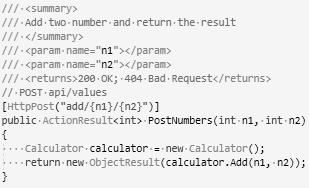
\includegraphics[width=0.45\linewidth]{Cap5/VSPostNumbers.png}
\caption{Estrutura do método \textit{PostNumbers}}
\label{Fig:Fig47}
\end{figure}

\begin{figure}[hbt!]
\centering
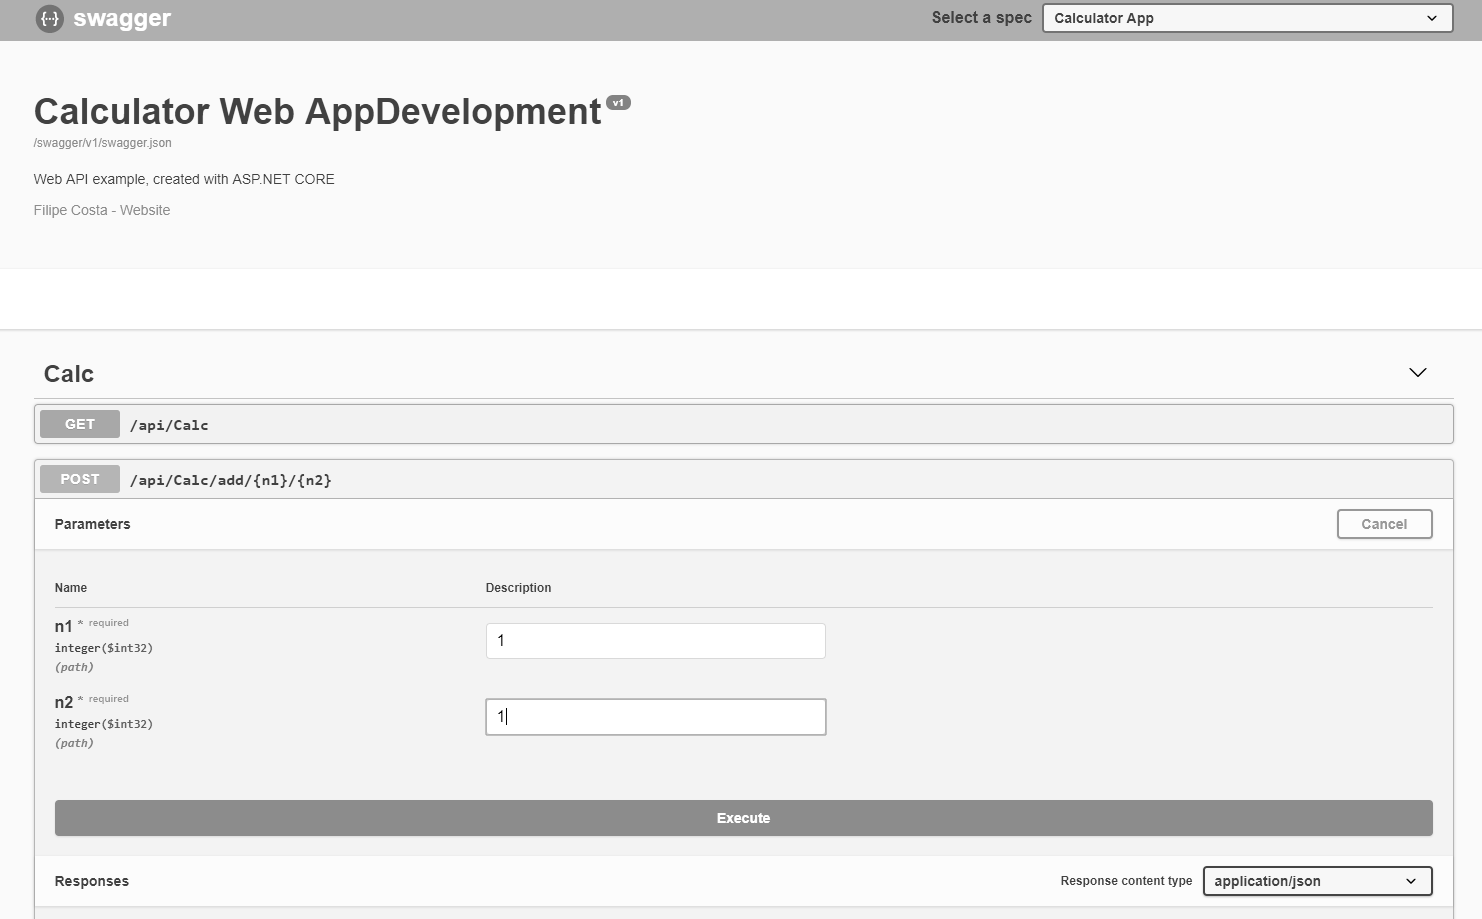
\includegraphics[width=0.8\linewidth]{Cap5/Swagger1.png}
\caption{Interface do \textbf{Swagger}}
\label{Fig:Fig48}
\end{figure}

\hspace{1cm}Para testar a \textbf{Web API} através da interface gráfica do \textbf{Swagger} deve ser executado (F5) o projeto e no \textit{browser}, após ser expandido o método \textit{POST}, clica-se em \textit{``Try it out''} de forma a que seja possível inserir dois números inteiros para executar a operação (\ref{Fig:Fig48}). Se a operação for bem sucedida é recebida uma resposta do servidor do \textbf{Kestrel} \cite{kestrel} com a resposta \textbf{200 OK} juntamente com o resultado da soma, caso contrário será retornada uma resposta do tipo \textbf{404 Bad Request}.

\begin{figure}[hbt!]
\centering
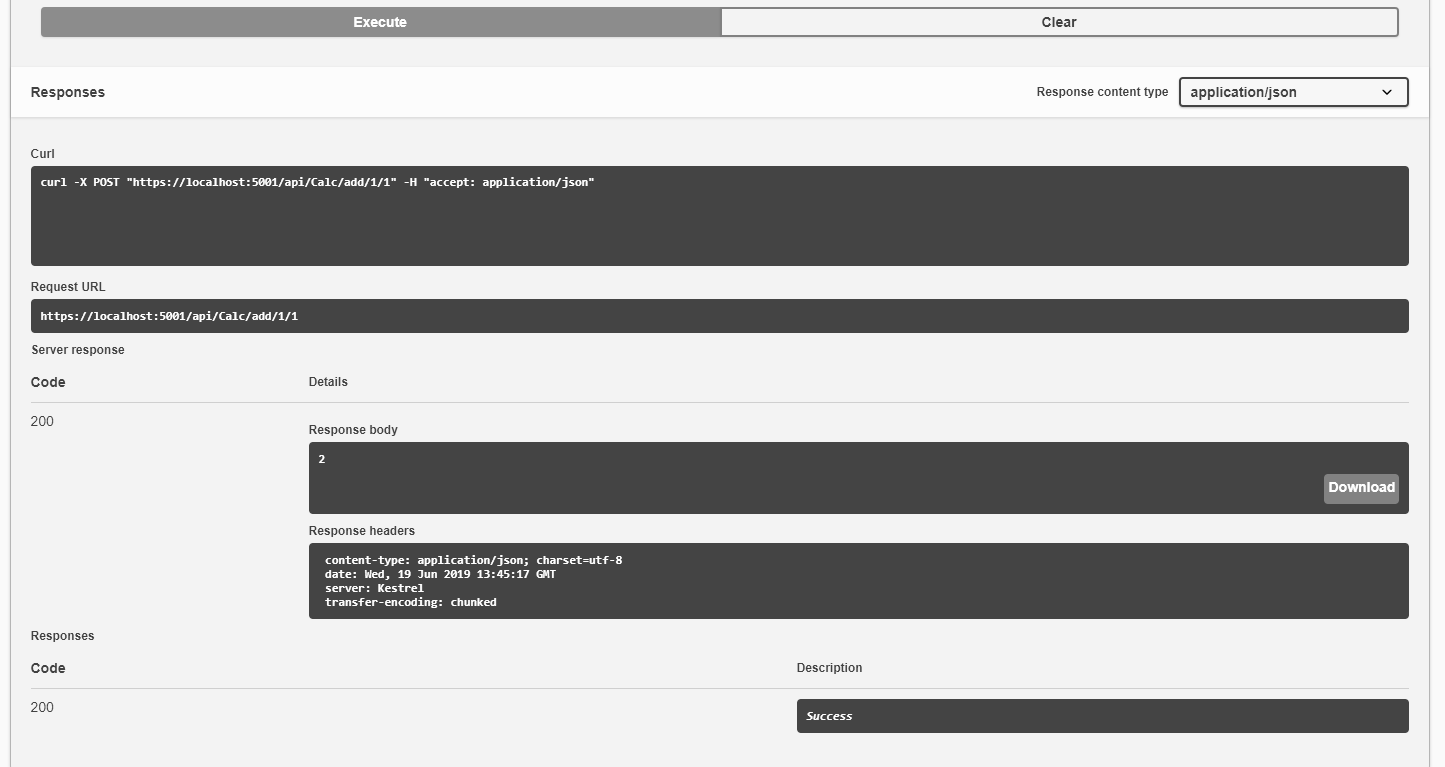
\includegraphics[width=0.8\linewidth]{Cap5/Swagger2.png}
\caption{Interface do \textbf{Swagger} com resposta \textbf{200 OK}}
\label{Fig:Fig49}
\end{figure}

\hspace{1cm}No caso foi retornada a resposta \textbf{200 OK} acompanhada pelo resultado da soma (\ref{Fig:Fig49}). A implementação da funcionalidade que foi desenvolvida, testada, empacotada e instalada na Web API está concluída. 

A próxima fase diz respeito aos testes de integração e performance.

\subsubsection{Criação dos testes de integração e performance}

\hspace{1cm}Os testes de integração e performance serão acompanhados pela criação de uma classe \textit{TestClientProvider}. Esta classe utiliza o servidor de testes da \textbf{Microsoft} -- o \textit{TestServer} -- para simular um cliente que faz pedidos à aplicação. O projeto de teste será criado em \textbf{xUnit} e vai incluir uma referência ao projeto da \textbf{Web API}. À semelhança dos testes unitários, os testes de integração -- que podem ou não incluir testes de performance -- seguem a mesma metodologia, \textit{Triple A}. No entanto, a estrutura dos testes de integração é ligeiramente mais complexa e, caso se pretenda incluir testes de performance, a sua complexidade aumenta. Para a implementação dos testes de integração serviram de apoio as páginas da documentação oficial da \textbf{Microsoft} sobre testes de integração \cite{microsoftintegrationtesting}, o blogue do \textbf{Andrew Lock} \cite{andrewlockblog} e alguns vídeos disponibilizados no canal \textbf{Dot Net Core Central} \cite{dotnetcorecentral} sobre criação de testes de integração.

\subsubsection{Pré-requisitos:}

\begin{itemize}
 \item xUnit (2.4.0);
 \item xUnit.runner.visualstudio (2.4.0);
 \item ModelClasses (1.0.3.4);
 \item FluentAssertions (5.6.0);
 \item Microsoft.AspNetCore.TestHost (2.2.0);
 \item Microsoft.AspNetCore.HttpsPolicy (2.2.0);
 \item Microsoft.AspNetCore.Diagnostics (2.2.0);
 \item Microsoft.AspNetCore.Mvc (2.2.0);
 \item Newtonsoft.Json (12.0.1);
\end{itemize}

\subsubsection{Objetivo dos testes de integração e performance}

\hspace{1cm}Os testes de integração são desenvolvidos quando pretendemos verificar as respostas de um pedido a um determinado \textit{endpoint}. Imaginemos que se pretende testar o comportamento de um método \textbf{POST}, semelhante aquele implementado na \textbf{Web API}, verificando que são efetivamente adicionados os dois números inteiros. Para tal, terá de se verificar que a resposta retornada é do tipo \textbf{200 OK} e que o resultado obtido é igual ao resultado esperado.

\hspace{1cm}Os testes de performance vão ser incluídos na execução dos testes de integração e terão como objetivo medir o seu tempo de execução. É necessário ter em conta que a primeira execução dos testes de integração é sempre mais demorada que as seguintes uma vez que, neste contexto, estará a ser inicializado o servidor de testes antes de ser criado um cliente. 

\begin{figure}[hbt!]
\centering
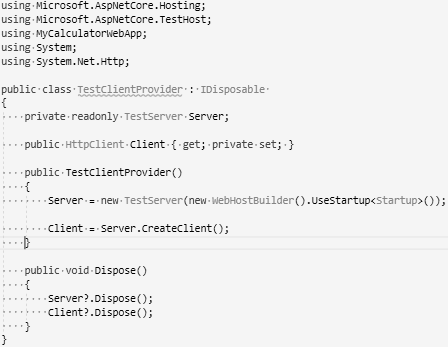
\includegraphics[width=0.7\linewidth]{Cap5/VSTestServer.png}
\caption{Estrutura do \textit{TestClientProvider}}
\label{Fig:Fig50}
\end{figure}

\hspace{1cm}Como dito anteriormente, para simular a criação do cliente utiliza-se a classe \textit{TestServer} que foi desenvolvida pela \textbf{Microsoft}. Desta forma, é criada uma nova classe, dentro do projeto de \textbf{xUnit}, chamada \textit{TestClientProvider} (\ref{Fig:Fig50}). Esta classe vai herdar as propriedades da classe \textit{IDisposable}, vai ter uma propriedade privada do tipo \textit{TestServer} -- que será o  servidor de testes -- e uma propriedade pública do tipo \textit{HttpClient} -- que será o cliente -- cujo objetivo será fazer pedidos à aplicação \textit{MyCalculatorWebApp}. Ainda dentro da classe vão constar dois métodos. O primeiro método será utilizado para criar o servidor de testes com a configuração da classe \textit{Startup.cs} e o cliente que lhe fará pedidos. O segundo método fará \textit{Dispose} ao cliente e ao servidor de testes.



\hspace{1cm}Para ser testada a integração do método \textit{POST}, a \textit{Theory} vai ter apenas um caso de teste -- chamado \textit{TestForResponseTypePOST} (\ref{Fig:Fig51}) -- com três parâmetros inteiros, \textit{n1}, \textit{n2} e \textit{result}. Na fase de \textit{Arrange} será instanciado um novo cliente da classe \textit{TestClientProvider}. De seguida, na fase de \textit{Act}, é dado inicio à contagem do tempo de execução do método \textit{POST} juntamente com o tempo da resposta do servidor. No final, na fase de \textit{Assert}, verifica-se que o tempo demorado é menor do que um valor pré-estabelecido (no caso dois segundos) e depois, com base nessa condição, são feitas duas verificações. É feita uma verificação ao tipo de resposta e outra verificação ao conteúdo da mensagem. Tal como é possível ver na figura \ref{Fig:Fig51}, uma das verificações é feita com o \textit{xUnit} ao passo que a outra é feita em \textit{FluentAssertions}.

\begin{figure}[hbt!]
\centering
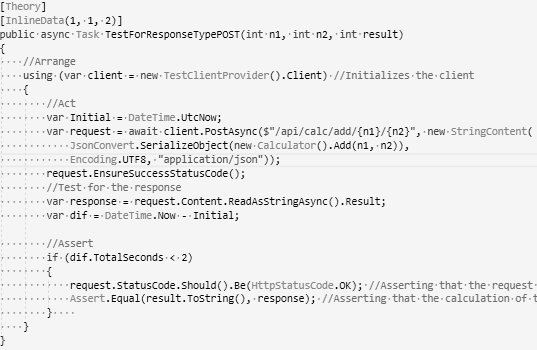
\includegraphics[width=0.7\linewidth]{Cap5/VSIntegrationTest.png}
\caption{Estrutura do \textit{TestForResponseTypePOST}}
\label{Fig:Fig51}
\end{figure}

\hspace{1cm}A próxima fase passará pela integração do código da \textbf{Web API} numa \textit{pipeline}, com análise estática e execução de testes de integração. Pode-se ou não integrar as notificações acerca do \textit{status} do \textit{job} com as plataformas de comunicação que a empresa utiliza, neste caso o \textbf{Slack}, mas o principal objetivo é fazer \textit{build} ao projeto da \textbf{Web API} e \textit{restore} às dependências do projeto.

\subsubsection{Configuração do \textit{job}}

\hspace{1cm}Partindo do pressuposto que o código da \textbf{Web API} foi publicado no \textbf{VCS}, serão repetidos os passos realizados na criação do \textit{job} anterior. No \textbf{Jenkins} será criado um \textbf{new item}, do tipo \textit{freestyle job}, podendo ser adicionada uma descrição. Depois será necessário adicionar a ligação ao \textbf{VCS}, a \textbf{GitLab Connection} que foi criada anteriormente, para que seja possível trazer para o \textbf{Jenkins} o código armazenado no repositório (\ref{Fig:Fig52}).

\begin{figure}[hbt!]
\centering
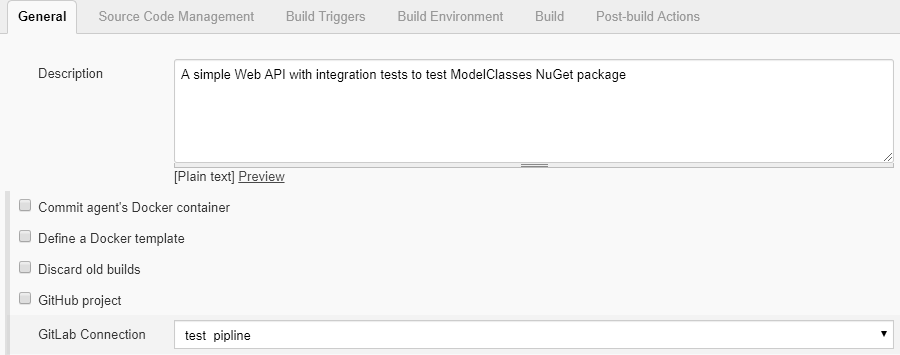
\includegraphics[width=0.9\linewidth]{Cap5/JenkinsGitLabConnection.png}
\caption{Configuração da descrição e do \textit{access token}}
\label{Fig:Fig52}
\end{figure}

\hspace{1cm}Em \textbf{Source Code Management} selecciona-se o repositório \textbf{GitLab} para onde foi publicado o código. Mais uma vez a comunicação entre o sistema de controlo de versões com \textbf{Jenkins} será feita via \textit{SSH}.

\hspace{1cm}Para que o processo de \textit{build} do \textit{job} que está a ser configurado esteja encadeado com o processo de \textit{build} do \textit{job} anterior será preciso fazer-se uma configuração na secção de \textbf{Build Triggers}. Para tal, é necessário selecionar a opção \textit{``Build after other projects are built''} (\ref{Fig:Fig53}) e, como se pretende que apenas seja feito um \textit{trigger} caso a \textit{build} anterior seja bem sucedida, selecciona-se também a opção \textit{``Trigger only if build is stable''}.

\begin{figure}[hbt!]
\centering
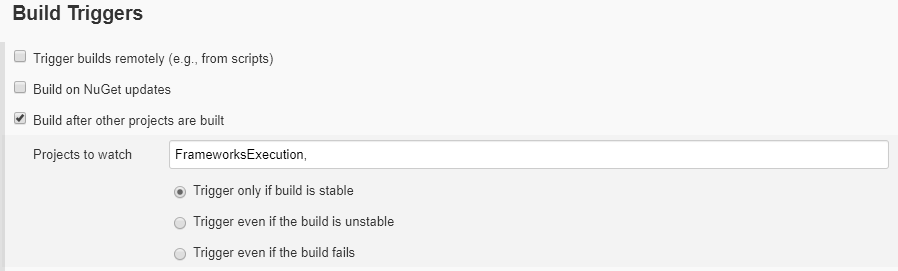
\includegraphics[width=0.9\linewidth]{Cap5/JenkinsBuildSecondPipelineAutomatically.png}
\caption{Configuração dos \textit{Build Triggers}}
\label{Fig:Fig53}
\end{figure}

\hspace{1cm}No próximo segmento, em \textbf{Build Environments}, é importante não esquecer de se selecionar a opção de \textit{``Delete workspace before build starts''}, para que seja apagado o \textit{workspace} criado pelo \textbf{Jenkins} antes do início de cada \textit{build}.

\hspace{1cm}Na fase de \textit{build} passa-se à configuração de um conjunto de instruções para integrar a análise estática, a \textit{build} à solução da \textbf{Web API}, a execução dos testes de integração e a interpretação do resultado dos testes, tal como no \textit{job} anterior. À semelhança daquilo que se fez, a integração da análise estática inicia-se através da instrução inicial \colorbox{gray}{\textcolor{white}{\$ dotnet SonarScanner.MSBuild.dll begin /k:``project-key''}} e termina-se com a instrução final \colorbox{gray}{\textcolor{white}{\$ dotnet SonarScanner.MSBuild.dll end}}. A \textit{build} ao projeto é feita com a instrução \colorbox{gray}{\textcolor{white}{\$ dotnet build project-path}} com a adição das opções \colorbox{gray}{\textcolor{white}{-{}-source http://package-source}} onde ``http://package-source'' será o repositório de \textbf{NuGet Packages}. Para se executarem os testes de integração utiliza-se o mesmo \colorbox{gray}{\textcolor{white}{\$ dotnet test project-path -{}-no-build -{}-logger trx}}. Na figura \ref{Fig:Fig54} vêm-se as instruções de \textit{build} à solução assim como de execução dos testes de integração.

\begin{figure}[hbt!]
\centering
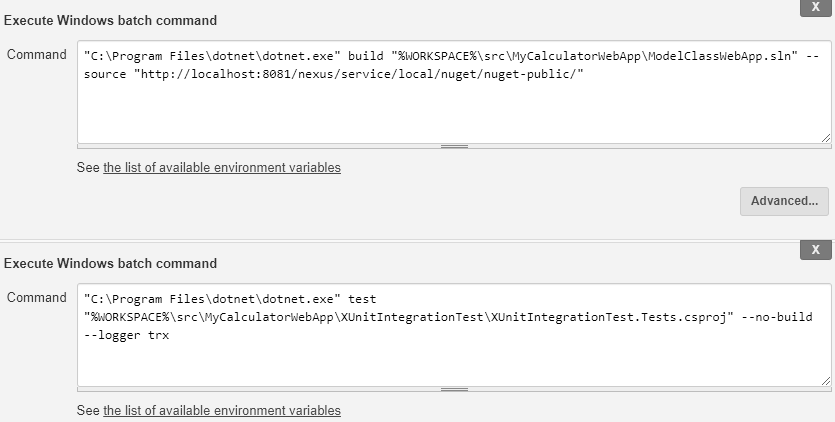
\includegraphics[width=0.9\linewidth]{Cap5/JenkinsBuildSecondPipelineBuildSteps.png}
\caption{Configuração dos \textit{Build Steps}}
\label{Fig:Fig54}
\end{figure}

\subsubsection{Integração com \textbf{Slack}}

\hspace{1cm}Para a integração do \textbf{Jenkins} com a plataforma de comunicação interna da empresa -- \textbf{Slack} -- é necessária a instalação do \textit{plugin} \textbf{Slack Notifications} (https://plugins.jenkins.io/slack). 

\hspace{1cm}Do lado do \textbf{Slack} a configuração é relativamente simples. Primeiro é necessário pedir um \textit{token} de acesso à plataforma de comunicação. Isto é feito através do painel de configuração das aplicações \textbf{Slack}. Neste painel (\ref{Fig:Fig55}) pode ser criado o canal com o qual a aplicação -- \textbf{Jenkins CI} -- vai comunicar o estado das \textit{builds} e é também aqui que se gera o \textit{token} de acesso à plataforma de comunicação. 

\begin{figure}[hbt!]
\centering
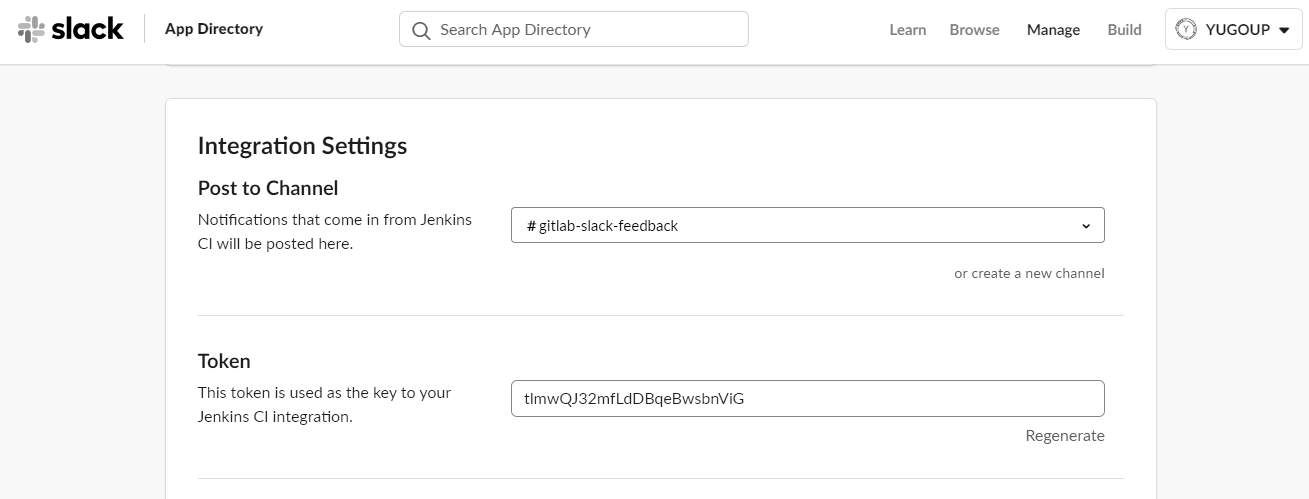
\includegraphics[width=0.9\linewidth]{Cap5/SlackConfiguration.png}
\caption{Configuração do \textbf{Jenkins CI}}
\label{Fig:Fig55}
\end{figure}

\hspace{1cm}Do lado do \textbf{Jenkins}, como se pode ver na figura \ref{Fig:Fig56}, antes da configuração da \textit{pipeline}, é necessário adicionar o \textit{token} de acesso gerado anteriormente, juntamente com o nome do canal para o qual será transmitida a informação.

\begin{figure}[hbt!]
\centering
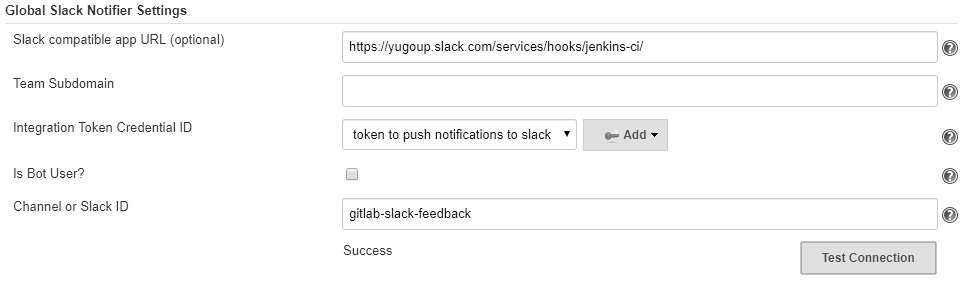
\includegraphics[width=0.9\linewidth]{Cap5/JenkinsSlackNotification.png}
\caption{Configuração do \textbf{Slack Notifier}}
\label{Fig:Fig56}
\end{figure}

\hspace{1cm}De seguida, e para finalizar a configuração das \textbf{Slack Notifications}, será necessário voltar ao \textit{job}. No \textit{job} é na fase de \textbf{Post-build Actions} que, para além de serem agregados todos dos resultados da execução dos testes, serão também adicionadas as \textit{Slack Notifications}. Aqui selecionam-se as opções pretendidas, desde notificações de sucesso/insucesso da \textit{build} até a informações sobre os \textit{commits} (\ref{Fig:Fig57}). 

\begin{figure}[hbt!]
\centering
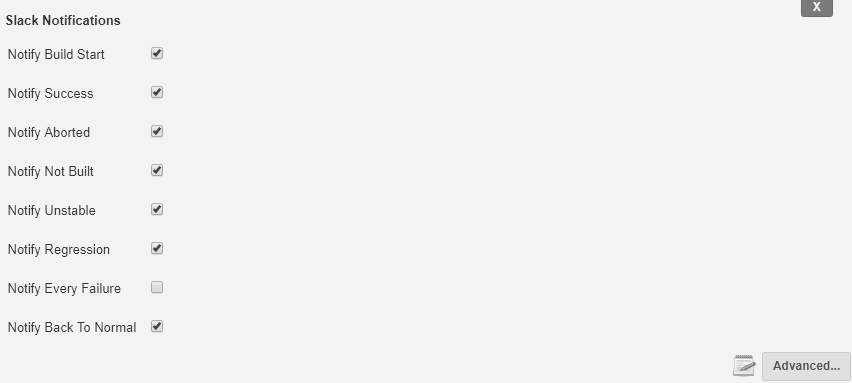
\includegraphics[width=0.9\linewidth]{Cap5/JenkinsPostBuildSlackNotifications.png}
\caption{\textit{Post-build action de \textbf{Slack Notification}}}
\label{Fig:Fig57}
\end{figure}

\hspace{1cm}Nesta fase a \textit{pipeline} contabiliza dois \textit{jobs}. O primeiro \textit{job} encarrega-se da automatização das fases de \textit{build}, \textit{static analysis}, \textit{unit testing}, \textit{packaging} e \textit{push} do módulo de soma para um repositório de artefactos. O segundo \textit{job} encarrega-se das fases de \textit{build}, \textit{static analysis}, \textit{integration testing} e notifica o developer acerca do estado da \textit{build} da \textbf{Web API}. A última fase da \textit{pipeline} envolve a criação de um \textit{job} com o propósito de automatizar a construção e publicação de uma imagem da aplicação. A imagem vai ser criada através de um ficheiro -- \textbf{Dockerfile} -- e a aplicação vai ser publicada através da utilização do \textbf{Docker}.

\subsection{Publicação da Web API}

\hspace{1cm}Para a publicação da aplicação vai ser utilizado o \textbf{Docker}. É através desta tecnologia de orquestração de \textit{containers} que será criada e publicada uma imagem da aplicação com recurso a registo privado de imagens. Com este registo privado podem ser geridas as imagens das aplicações que são criadas sem que mais ninguém tenha acesso. Caso estivessem no registo público do \textbf{Docker}, estariam disponíveis para uso público.

\subsubsection{Criação de um \textit{Dockerfile}}

\hspace{1cm}O \textbf{Dockerfile} é o documento que vai ser utilizado para executar um conjunto de instruções que vão gerar uma versão de \textit{Release} da \textbf{Web API} que foi criada (\ref{Fig:Fig72}). Para a imagem da \textbf{Web API} estar totalmente funcional é necessário copiar os ficheiros \textbf{.csproj} para a \textit{working directory} -- neste caso \textbf{/app} -- para depois resolver as dependências do projeto que estão guardadas no repositório de artefactos. De seguida, a pasta com as dependências resolvidas é copiada para a \textit{working directory}. Depois, novamente a partir da pasta da \textbf{Web API}, é feita \textit{build} à solução com a configuração de \textbf{Release} e com o \textit{output} a ser enviado para a pasta \textbf{/app}. 

\begin{figure}[hbt!]
\centering
\includegraphics[width=0.9\linewidth]{Cap5/DockerfileCalculator.png}
\caption{Estrutura do \textit{Dockerfile}}
\label{Fig:Fig72}
\end{figure}

\hspace{1cm}A partir do resultado da instrução gerada na fase de \textit{build} vai publicar-se o conteúdo gerado para a pasta \textbf{/app} com a configuração de \textit{Release}. Para finalizar, a partir da imagem base, volta-se novamente para a pasta \textbf{/app}, copia-se o conteúdo da instrução anterior (\textit{publish}) para a pasta atual e passa-se o \textit{entrypoint} que é a \textit{dynamically linked library} da \textbf{Web API}.

\hspace{1cm}Após a criação da primeira imagem vai automatizar-se todo o processo de geração da mesma na \textit{pipeline} de integração contínua. Claro está que para tal será necessário recorrer ao \textit{script} gerado anteriormente.

\subsubsection{Criação do job}

\hspace{1cm}O \textit{workflow} inicial do novo \textit{job} é ligeiramente diferente do anterior. Até à fase de \textbf{Build}, não existe qualquer alteração nas configurações. Contudo, quando se executam as instruções necessárias para automatizar o processo de geração, publicação e lançamento da imagem, terão de utilizar-se dois tipos de \textit{build steps} distintos. Até agora têm sido utilizado maioritariamente \textbf{Windows batch command} mas, para este caso, terá de se utilizar \textbf{shell scripts}. 

\subsubsection{Setup do ambiente}

\hspace{1cm}Para o \textbf{setup} ao ambiente irá fazer-se \textit{build} à solução da \textbf{Web API}. À semelhança daquilo que foi feito no \textit{script}, também terá de ser indicada na instrução a \textit{source} dos \textbf{NuGet Packages} (\ref{Fig:Fig73}). O primeiro \textbf{Build step} vai definir o \textit{WORKSPACE} dentro do \textbf{Jenkins}. Com o ambiente definido será necessário entrar na pasta onde está presente o \textbf{Dockerfile}. A instrução para mudar de diretorias no \textbf{Windows} é \colorbox{gray}{\textcolor{white}{\$ cd directory-path}} originado de \textit{change directory}. 

\begin{figure}[hbt!]
\centering
\includegraphics[width=0.9\linewidth]{Cap5/JenkinsBuildModelClassWebApp.png}
\caption{Instrução de \textit{build} à solução}
\label{Fig:Fig73}
\end{figure}

\subsubsection{Criação, publicação e lançamento da imagem da Web API}

\hspace{1cm}Para que se tenha uma ideia de como é gerada, publicada e instanciada uma imagem de \textbf{Docker} é importante que seja lida a documentação sobre estas instruções na página oficial do \textbf{Docker} sobre imagens \cite{dockerimages} e \textit{containers} \cite{dockercontainers}. A sequência cronológica de instruções de publicação de uma aplicação através da utilização de \textbf{Docker CLI} pode ser vista na figura \ref{Fig:Fig74}.

\begin{figure}[hbt!]
\centering
\includegraphics[width=0.9\linewidth]{Cap5/JenkinsGenerateDockerImage.png}
\caption{Criação, publicação e lançamento da imagem da Web API}
\label{Fig:Fig74}
\end{figure}

A imagem da \textbf{Web API} vai ser gerada com uma \textbf{tag} do endereço local do serviço de \textit{registry} seguido pelo seu nome \colorbox{gray}{\textcolor{white}{\$ docker build -t registry-address/image .}}. O servico de \textit{registry} é uma aplicação \textit{server side stateless} escalável que nos permite armazenar e distribuir imagens \textbf{Docker} \cite{dockerregistry}. Existem outras alternativas para armazenamento de imagens, no entanto a implementação implicaria a emissão de um certificado \textbf{SSL self-signed} e para o caso pretende manter-se o processo o mais simples possível.

A próxima instrução será utilizada para colocar a imagem dentro do \textbf{Docker registry}. Para tal, utiliza-se \colorbox{gray}{\textcolor{white}{\$ docker push registry-address/image}} e, para garantir que a instrução funciona corretamente, é necessário verificar que a \textbf{tag} da imagem é igual à \textbf{tag} da instrução anterior. 

De seguida, remove-se a imagem que foi criada na máquina com recurso à instrução \colorbox{gray}{\textcolor{white}{\$ docker image rm registry-address/image}}. Pode ser necessário utilizar a opção \colorbox{gray}{\textcolor{white}{-{}-force}} para que a imagem seja completamente removida do \textbf{Docker} local. Depois, para publicar num \textit{container} a \textbf{Web API} a partir da imagem armazenada no registo, será utilizada a instrução \colorbox{gray}{\textcolor{white}{\$ docker container run [options] image}} juntamente com algumas opções para lançar o \textit{container} na porta \textbf{8123}.

\subsubsection{Pedidos à Web API}

\hspace{1cm}Depois de publicada a imagem vão ser feitos alguns pedidos à aplicação. Para tal, são utilizadas as instruções do \textbf{curl} (https://curl.haxx.se/) tal como pode ser visto na figura \ref{Fig:Fig75}. Para garantir que a aplicação é devidamente publicada e só depois são feitos os pedidos aguarda-se durante 15 segundos com a instrução \colorbox{gray}{\textcolor{white}{\$ sleep 15}}. Só depois são executadas as instruções para os pedidos \textbf{GET} e \textbf{POST} sendo que o \textit{output} pode ser verificado diretamente no \textbf{Jenkins}. 

\begin{figure}[hbt!]
\centering
\includegraphics[width=0.9\linewidth]{Cap5/JenkinsRequestWebAPI.png}
\caption{\textit{Requests} à Web API}
\label{Fig:Fig75}
\end{figure}

\hspace{1cm}Depois de feitos os \textit{requests} e validado o comportamento da \textbf{Web API}, irá ser parado o \textit{container} que foi lançado através da utilização da instrução de paragem \colorbox{gray}{\textcolor{white}{\$ docker container stop container-name}} (\ref{Fig:Fig76}).

\begin{figure}[hbt!]
\centering
\includegraphics[width=0.9\linewidth]{Cap5/JenkinsStopDockerContainer.png}
\caption{Instrução de paragem do \textit{container}}
\label{Fig:Fig76}
\end{figure}

\section{Considerações}

\hspace{1cm}Recapitulando o trabalho feito neste capítulo, que envolveu:

\begin{itemize}
 \item Configuração de um sistema de controlo de versões;
 \item Desenvolvimento um conjunto de testes unitários para validação do funcionamento do módulo de soma;
 \item Configuração um orquestrador de processos (\textbf{Jenkins});
 \item Configuração de um \textit{job} para automatizar as fases de \textit{build}, \textit{static analysis}, \textit{test}, \textit{pack} e \textit{push} de um \textbf{NuGet Package} para um repositório de artefactos;
 \item Descrição do processo de desenvolvimento de uma \textbf{Web API};
 \item Configuração de um \textit{job} para automatizar as fases de \textit{build}, \textit{static analysis}, \textit{integration testing} e notificação do \textit{developer} acerca do estado da \textit{build} e dos detalhes da \textbf{Web API};
 \item Descrição do processo de geração, publicação e lançamento de uma imagem da \textbf{Web API};
 \item Configuração de um \textit{job} para automatizar a fase de \textit{build}, \textit{publish} e \textit{run} da imagem \textbf{Docker} da aplicação;
\end{itemize}

\hspace{1cm}O último passo consiste na criação de um ficheiro de composição dos serviços. Este ficheiro, semelhante ao da figura (\ref{Fig:Fig96}), iria conter dois serviços da \textbf{Web API} que foi criada, com a adição de um serviço de \textit{load balancing} para distribuição dos pedidos. Para fazer a distribuição dos pedidos à aplicação por dois \textit{containers} diferentes foi utilizado como \textit{Web Server} o \textbf{Nginx} (https://www.nginx.com/).

\begin{figure}[hbt!]
\centering
\includegraphics[width=0.43\linewidth]{Cap5/DockerComposeCalculator.png}
\caption{Estrutura do ficheiro \textit{docker-compose.yml}}
\label{Fig:Fig96}
\end{figure}

\hspace{1cm}Em termos de \textit{workflow} a \textbf{Web API} construída incorpora três fases de desenvolvimento. A primeira fase é a fase de \textit{development} onde se desenvolveu o módulo de soma através de práticas de \textbf{TDD}. Os testes são incorporados mais tarde numa \textit{pipeline} de integração contínua, são analisados pelo servidor de automação e, caso sejam bem-sucedidos, é gerado um artefacto daquele módulo que posteriormente será colocado no repositório de artefactos. 

\hspace{1cm}Na fase seguinte o módulo de soma foi utilizado por uma \textbf{Web API} desenvolvida para se verificar que os testes de integração podiam ser feitos através da utilização de uma tecnologia da \textbf{Microsoft}, o \textit{TestServer}. Os testes de integração também testam a performance da aplicação, mas é necessário ter em conta que a primeira execução vai ser sempre mais lenta dado que é necessário inicializar o servidor de testes.

\hspace{1cm}O \textbf{Jenkins} produz depois um \textit{report} detalhado da análise dos testes unitários e de integração que é apresentado ao utilizador para fins estatísticos.

\hspace{1cm}Na terceira fase de desenvolvimento -- a fase de \textit{staging} -- é produzido o \textbf{Dockerfile} que é utilizado para gerar uma imagem. Esta imagem, que no fundo é a versão de \textit{release} (executável) da aplicação, vai ser publicada no registo privado do \textbf{Docker} que foi criado para servir de repositório de imagens. Ainda neste fase, a imagem da aplicação é lançada dentro de um \textit{container} e são feitos dois pedidos à aplicação para verificar que funciona de forma correta. Caso estes pedidos retornem \textit{StatusCodes} diferentes do esperado a aplicação não estará a funcionar como é esperado e requer investigação.

\hspace{1cm}Na última fase -- \textit{Pre-live} -- coloca-se a imagem da aplicação criada, juntamente com uma imagem do \textit{load balancer}, dentro de um ficheiro \textbf{docker-compose.yml}.

\hspace{1cm}O próximo passo é a criação de uma imagem funcional de um serviço composto por uma arquitetura semelhante aquela utilizada pela empresa no desenvolvimento dos seus serviços. Depois da apresentação da solução é ainda apresentado um conjunto de serviços que o \textbf{Docker} disponibiliza.

